\chapter{Ecuaciones Lineales de Segundo Orden}
%\date{}

%\begin{document}




%\tableofcontents




\section{Introducción}


\begin{quote}
Me convertí en ateo porque como estudiante de  post-grado en física cuántica, la vida parecía ser reducible a ecuaciones diferenciales de segundo orden. Matemáticas, 
química y física tenían todo y yo no veo ninguna necesidad de ir más allá de eso.
\end{quote}
\begin{flushright}
Francis Collins
\end{flushright}




\begin{definicion}[Ecuación lineal general de segundo orden]{}
 \boxedeq{\frac{d^2y}{dx^2}+p(x)\frac{dy}{dx}+q(x)y=r(x),}{ec_2_gen}
donde $p,q,r$ son funciones definidas en un intervalo $I=(a,b)$ de $\rr$ con valores en $\rr$.Si $r\equiv 0$ se llama homogénea
\boxedeq{\frac{d^2y}{dx^2}+p(x)\frac{dy}{dx}+q(x)y=0,}{ec_2_gen_hom}
\end{definicion}







\begin{teorema}[Teorema de existencia y unicidad de soluciones]{}
Supongamos $p,q,r$ continuas y acotadas sobre $I$. Sean $x_0\in I$ e $y_0,y_1\in\rr$ dados. Entonces existe una única solución del PVI
\[\left\{
\begin{array}{l l l}
\frac{d^2y}{dx^2}+&p(x)\frac{dy}{dx}+q(x)y=r(x),&x\in I\\
y(x_0)&=y_0&\\
y'(x_0)&=y^1_0&\\
\end{array}\right.
\]
\end{teorema}
\begin{proof} Es un caso particular del Teorema Picard- Lindelöf. Más específicamente de un ejercicio que se presentó en la actividad práctica. Llamando $z=y'(x)$ el PVI propuesto se convierte en un PVI asociado a un sistema de ecuaciones
\[\left\{
\begin{array}{l l l}

y'(x)&= z(x)\\
z'(x)&= -p(x)z(x)-q(x)y+r(x),\\
y(x_0)&=y_0\\
z(x_0)&=y^1_0\\
\end{array}\right.
\]

Es un sistema de la forma $w'(x)=f(x,w(x))$ donde $w(x)=(y(x),z(x))$ y $f(x,w)=(z,-p(x)z-q(x)y+r(x)$. Vamos a chequaer que $f$ es Lipschitz respecto a la segunda variable  en $I\times \rr^2$. Si $(x,w_0),(x,w_1)\in I\times \rr^2$  ($w_0=(z_0,y_0)$ y $w_1=(z_1,w_1)$) entonces:
\[
\begin{split}
  \|f(x,w_1-f(x,w_2)\|&\leq \sqrt{(z_1-z_0)^2+  (p(x)(z_1-z_0)+q(x)(y_1-y_0)^2}\\
  &\leq
 C\|w_1-w_0\|,
\end{split}
\]
para una constante apropiada $C$ que depende de una cota de $|p(x)|,|q(x)|$, $x\in I$.
Cómo $f$ es Lipschitz respecto a la segunda variable en todo $\rr^2$, el sistema tiene una solución definida en todo $I$.




\end{proof}


\section{Estructura del conjunto de soluciones}
\begin{teorema}{}
Si $y_1$ e $y_2$ son soluciones de \eqref{ec_2_gen_hom} y $c_1,c_2\in\rr$ entonces $c_1y_1+c_2y_2$ es solución. Vale decir, el conjunto de soluciones
es un espacio vectorial. En particular $y\equiv 0$ es una solución, a la que llameremos \emph{trivial}.
\end{teorema}

\begin{proof}
 El operador
\[L[y]:=y''+py'+qy\]
es lineal, por consiguiente
$L[c_1y_1+c_2y_2]=c_1L[y_1]+c_2L[y_2]=0.$
\end{proof}


\begin{teorema}{}
 Supongamos que $y_p$ es una solución particular de \eqref{ec_2_gen} y que $y_g=y_g(x,c_1,c_2)$ es una solución
general de \eqref{ec_2_gen_hom}. Entonces $y=y_p+y_g$ es solución general de \eqref{ec_2_gen}.
\end{teorema}



\begin{proof}
El operador
\[L[y]:=y''+py'+qy\]
es lineal, por consiguiente
$L[y_g+y_p]=L[y_g]+L[y_p]=0+r=r.$
Recíprocamente supongamos $y$ solución de $L[y]=r$, entonces
$L[y-y_p]=L[y]-L[y_p]=r-r=0.$
Luego debe haber $c_1$ y $c_2$ con $y(x)-y_p(x)=y_g(x,c_1,c_2)$.

\end{proof}


Volviendo a las ecuaciones homogéneas, supongamos que tenemos dos soluciones de \eqref{ec_2_gen_hom} $y_1$ e $y_2$. Entonces la expresión
\begin{equation}\label{comb_lin}
c_1y_1+c_2y_2,\quad c_1,c_2\in\rr
\end{equation}
es solución también. Notar que en la expresión aparecen dos constantes y habíamos dicho que era de esperar que la solución general de una ecuación de orden 2 contuviese
precisamente dos constantes de integración. De modo que podemos conjeturar que \eqref{comb_lin} es solución general de \eqref{ec_2_gen_hom}.
Hay una situación especial, si, por ejemplo, $y_1=ky_2$, $k\in\rr$,entonces $c_1y_1+c_2y_2=(c_1k+c_2)y_2=cy_2$. Vale decir la combinación lineal \eqref{comb_lin}
termina siendo sólo combinación lineal de la función $y_2$ y por ende siendo esencialmente una expresión uniparamétrica.

\begin{definicion}[Independencia lineal]{}
 Un conjunto finito de funciones $\{y_1,\ldots,y_n\}$ se dirá linealmente independiente sobre un conjunto $I$,
si la única solución de $c_1y_1(t)+\cdots+c_ny_n(t)=0$, para $t\in I$, es $c_1=c_2=\cdots=c_n=0$.
\end{definicion}




\begin{definicion}[Definición wronskiano]{}
 Dadas $n$ fuciones $\{y_1,\ldots,y_n\}$ con dominio $I$, el wronskiano $W(x)=W(y_1,y_2,\ldots,y_n)(x)$ de estas funciones en un punto $x\in I$ se define por
\boxedeq{W(x)=\det\begin{pmatrix}
y_1(x) & y_2(x) & \cdots &y_n(x)\\
y_1'(x) & y_2'(x) & \cdots &y_n'(x)\\
\vdots & \vdots &\ddots& \vdots\\
y_1^{(n-1)}(x) & y_2^{(n-1)}(x) & \cdots &y_n^{(n-1)}(x)\\
\end{pmatrix}}{wronskiano}
\end{definicion}




\begin{lema}[Propiedades Wronskiano I]
 Sea $\{y_1,\ldots,y_n\}$ un conjunto de $n$ funciones. Si existe un $x_0\in I$ con $W(x_0)\neq 0$ entonces $\{y_1,\ldots,y_n\}$ son
linealmente independientes
\end{lema}


\begin{proof} Supongamos que $c_1y_1+\cdots+c_ny_n\equiv 0$. Derivando $n-1$ veces esta igualdad y evaluando el resultado en $x_0$ obtenemos
\[
\begin{split}
c_1y_1(x_0)+\cdots+c_ny_n(x_0)&=0\\
c_1y_1'(x_0)+\cdots+c_ny'_n(x_0)&=0\\
\vdots \quad& \quad\vdots\\
c_1y_1^{(n-1)}(x_0)+\cdots+c_ny^{(n-1)}_n(x_0)&=0\\
\end{split}
\]
Las igualdades anteriores dicen que el vector $(c_1,\ldots,c_n)^t$ pertenece al nucleo de la matriz
\[
\begin{pmatrix}
y_1(x_0) & y_2(x_0) & \cdots &y_n(x_0)\\
y_1'(x_0) & y_2'(x_0) & \cdots &y_n'(x_0)\\
\vdots & \vdots &\ddots& \vdots\\
y_1^{(n-1)}(x_0) & y_2^{(n-1)}(x_0) & \cdots &y_n^{(n-1)}(x_0)\\
\end{pmatrix}
\]
Como por hipótesis la matríz es no singular, debe ocurrir que $c_1=c_2=\cdots c_n=0$.
\end{proof}

\begin{teorema}[Teorema. Propiedades wronskiano II, Fórmula de Abel]{}
 Supongamos que $y_1$ e $y_2$ son solución de
\begin{equation}\label{eq2orden}\frac{d^2y}{dx^2}+p(x)\frac{dy}{dx}+q(x)y=0,\quad x\in I=(a,b)\end{equation}
Entonces existe $c\in\rr$ que satisface
\boxedeq{W(y_1,y_2)(x)=ce^{-\int p dx}.}{formu_abel}
Esta expresión se denomina \href{http://en.wikipedia.org/wiki/Abel's_identity}{fórmula de Abel}. En particular vale que
\[\exists x_0\in I: W(x_0)\neq 0 \Longleftrightarrow \forall x\in I: W(x)\neq 0 .\]
\end{teorema}

\begin{proof} Tenemos que
\[W(x)=y_1(x)y_2'(x)-y_1'(x)y_2(x).\]
Derivando y usando \eqref{eq2orden}
\[\begin{split}W'(x)&=y_1y_2''-y_1''y_2\\
&=y_1(-py_2'-qy_2)-y_2(-py_1'-qy_1)\\
&=-pW.
\end{split}
\]
Vale decir $W$ resuelve la ecuación $W'=-pW$ la cual es facilmente resoluble, mostrando su resolución que se satisface \eqref{formu_abel}
\end{proof}

\begin{teorema}[Propiedades wronskiano III]{}
 Sean $y_1$ e $y_2$ soluciones de \eqref{eq2orden}. Entonces son equivalentes
\begin{enumerate}
\item\label{item1} $y_1$ e $y_2$ son linealmente indepenientes en $I$.
\item\label{item2} $W(y_1,y_2)(x)\neq 0$ para todo $x\in I$.
\end{enumerate}
\end{teorema}


\begin{proof} Que \ref{item2} implica \ref{item1} es consecuencia de la propiedad del wronskiano I.
Veamos que \ref{item1} implica \ref{item2}. Supongamos que exista un $x_0$ con $W(x_0)=0$. Esto quiere decir que una de las columnas
de la matríz wronskiana en $x_0$ es múltiplo de la otra. Supongamos que $y_2(x_0)=ky_1(x_0)$ e $y'_2(x_0)=ky'_1(x_0)$. Esto quiere decir que $y_2$ y $ky_1$
resuelven el mismo pvi. Por lo tanto $y_2(x)=ky_1(x)$ para todo $x$. Lo que nos dice lo contrario de \ref{item1}
\end{proof}


\begin{teorema}[Estructura del conjunto de soluciones, ecuación  homogénea]{}
 Si $y_1$ e $y_2$ son soluciones linealmente independientes de
\[\frac{d^2y}{dx^2}+p(x)\frac{dy}{dx}+q(x)y=0,\quad x\in I=(a,b)\]
entonces
\boxedeq{ y(x,c_1,c_2)=c_1y_1+c_2y_2}{comb_lin2}
es solución general.
\end{teorema}

\begin{proof} Que la expresión \eqref{comb_lin2} es solución ya lo hemos dicho. Restaría ver que cualquier solución se escribe como en \eqref{comb_lin2}.
Sea $y$ cualquier solución y $x_0\in I$. La matriz wronskiana
\[\begin{pmatrix}
y_1(x_0) & y_2(x_0)\\
y'_1(x_0) & y'_2(x_0)\\
\end{pmatrix}
\]
Es no singular dado que el determinante es no nulo. Por este motivo el sistema
\[ \begin{split}
c_1 y_1(x_0) + c_2y_2(x_0) &=y(x_0)\\
c_1y'_1(x_0) + c_2y'_2(x_0) &=y'(x_0)\\
\end{split}
\]
tiene solución para $c_1$ y $c_2$. De este modo vemos que la función $c_1y_1+c_2y_2$ resuelve el PVI
\[\left\{
\begin{array}{l l l}
\frac{d^2z}{dx^2}+&p(x)\frac{dz}{dx}+q(x)z=0,&x\in I\\
z(x_0)&=y(x_0)&\\
z'(x_0)&=y'(x_0)&\\
\end{array}.\right.
\]
Evidentemente $y$ es solución también, por el Teorema de Existencia y Unicidad vemos que $y=c_1y_1+c_2y_2$ \end{proof}

\section{Reducción de orden}

Como conclusión de los anterior, vemos que si queremos resolver \eqref{eq2orden} debemos conseguir dos soluciones linealmente independientes.
Suponiendo que ya contamos con una solución no trivial vamos a describir un método
que posibilita encontrar otra solución $y_2$ linealmente independiente de $y_1$.
El método consiste en proponer que $y_2$ se escribe
\[\boxed{y_2(x)=v(x)y_1(x)}.\]
Sustituyendo este ansatz en la ecuación
\[
\begin{split}
0&=y_2''+py_2'+qy_2\\
&=y_1v''+2v'y_1'+vy_1''+pv'y_1+pvy_1'+qvy_1\\
&=y_1 v''+(2y_1'+py_1)v'+v(y_1''+py_1'+qy_1)\\
&=y_1 v''+(2y_1'+py_1)v'
\end{split}
\]
La fórmula anterior es nuevamente una ecuación de segundo orden para $v$,
pero en este caso afortunadamente contamos con herramientas para resolverla puesto que se trata de una ecuación donde la
variable dependiente $v$ no aparece explícitamente, sino que aparecen sus derivadas $v'$ y $v''$. Hay que intentar la sustitución $w=v'$.
Luego
\[
y_1w'+(2y_1'+py_1)w=0
\]
Recordar que $y_1$ la asumimos conocida, así $2y_1'+py_1$ es también una función conocida. La ecuación es una ecuación lineal homogénea de primer orden.
Usando la fórmula para resolver este tipo de ecuación, obtenemos
\[w(x)=Ce^{-\int \frac{y_1'}{y_1}+p dx}=Ce^{-2\ln|y_1|}e^{-\int p dx}=C\frac{1}{y_1^2}e^{-\int p dx} \]
Es suficiente encontrar sólo una función $v$, de allí podemos tomar $C=1$.
\boxedeq{w(x)= \frac{1}{y_1^2}e^{-\int p dx}\Longrightarrow v(x)= \int \frac{1}{y_1^2}e^{-\int p dx}dx }{reduc_orden}


Otra manera de testear la independencia lineal de dos funciones $y_1$ e $y_2$ es notar que si fueran linealmente dependientes e $y_1\neq 0$
en un conjunto $J\subset I$ entonces $y_2/y_1$
sería constante.
Luego uno chequearía independencia si comprobase que $y_2/y_1$ no es constante en algún subdominio $J\subset I$.
En el caso anterior $y_2/y_1=v$, luego
deberíamos tener $v$ no constante sobre algún subconjunto $J$. Pero $v$ constante implicaría $y_1^{-2}e^{-\int pdx}=0$ y esto claramente no ocurre. De modo que por el
método anterior encontramos dos soluciones independientes.

\section{Ecuaciones homogéneas con coeficientes constantes}

Consideramos la ecuación
\boxedeq{y''+py'+qy=0,\quad p,q\in\rr}{2orden_coef_ctes}
Propongamos una solución de la forma
\[\boxed{y(x)=e^{\lambda x},\quad \lambda\in\mathbb{C}}\]
Reemplazando en la ecuación
\[(\lambda^2+\lambda p+q)e^{\lambda x}=0.\]
Se debe satisfacer la llamada \emph{ecuación característica}
\boxedeq{\lambda^2+p\lambda+q=0}{ecua_carac}
Tenemos tres casos acorde al valor de $\Delta:=p^2-4q$

\begin{enumerate}

\item \noindent \textbf{ $\b{\Delta=p^2-4q>0}$, raices reales distintas $\b{\lambda_1$, $\lambda_2}$}. Este es el caso más sencillo de todos, obtenemos las soluciones
\[y_1(x)=e^{\lambda_1 x}\quad\text{y}\quad y_2(x)=e^{\lambda_2 x}.\]
Para chequear la independencia
\[\frac{y_2}{y_1}=e^{(\lambda_2-\lambda_1)x}\neq\text{cte}.\]
Luego
\boxedeq{y(x,c_2,c_2)=c_1e^{\lambda_1 x}+c_2e^{\lambda_2 x}.}{sol_gen1}
es solución general


\item \noindent  \textbf{$\b{\Delta=p^2-4q<0}$, raices complejas conjugadas $\lambda_1=\mu+i\nu$, $\lambda_2=\mu-i\nu$, $\mu,\nu\in\rr$}.
Proponemos una solución de la forma
\[
y(x)=e^{\mu x}v(x)
\]
Hagamos los cálculos con \texttt{SymPy}





\begin{lstlisting}
>>> x,p,q=symbols('x,p,q')
>>> v=Function('v')(x)
>>> y=exp(-p/2*x)*v
>>> ecua=y.diff(x,2)+p*y.diff(x)+q*y
>>> simplify(ecua/exp(-p/2*x))

\end{lstlisting}

\[-\frac{p^{2}}{4} v{\left (x \right )} + q v{\left (x \right )} + \frac{d^{2}}{d x^{2}}  v{\left (x \right )}=0
 \]

Como $\nu^2:=-\frac{1}{4}(p^2-4q)>0$, $v$ resuelve  la ecuación del oscilador armónico con frecuencia $\nu$. Recordar que la solución general
para $v$ es
\[v(x)=C_1\cos \nu x +C_2\sen \nu x,\]
y de allí
\boxedeq{y(x)=e^{\mu x}\left\{C_1\cos \nu x +C_2\sen \nu x\right\}}{sol_gen_2caso}

Seguidamente presentamos las gráficas de las soluciones para distiontos valores de $\mu$.

\begin{center}
 \begin{tabular}{c c c}
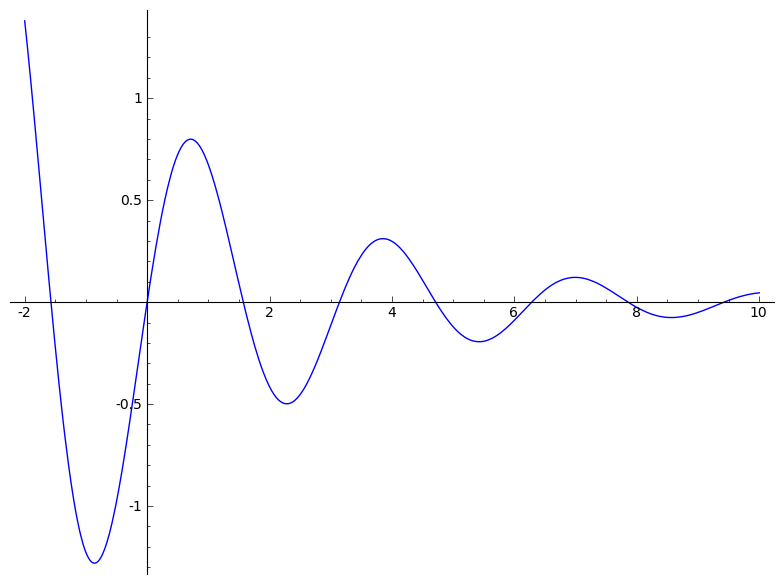
\includegraphics[scale=.1]{imagenes/mu_neg.png} & 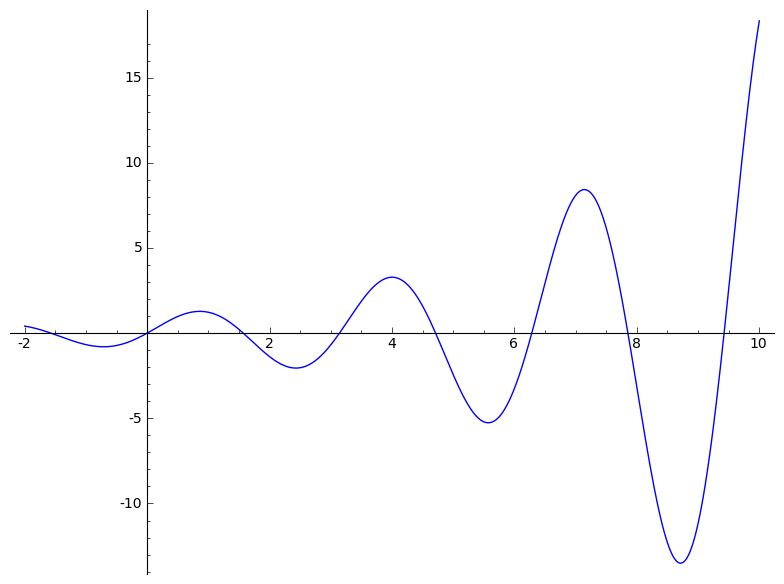
\includegraphics[scale=.1]{imagenes/mu_pos.png} &
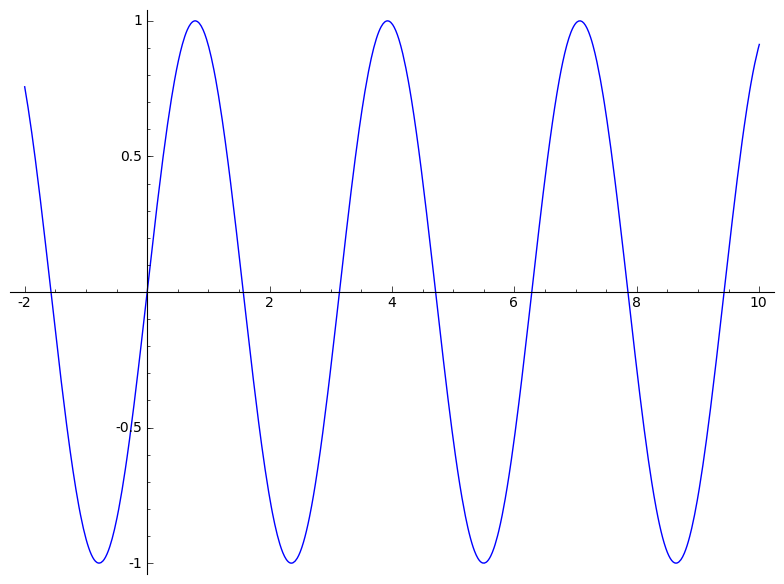
\includegraphics[scale=.1]{imagenes/mu_cero.png}\\
$\mu<0$ & $\mu>0$ & $\mu=0$\\
\end{tabular}

\end{center}








\item \noindent\textbf{ $\b{\Delta=p^2-4c=0}$, raices iguales }. Conocemos una solución $\boxed{y_1=e^{-\frac{p}{2}x}}$. Podemos hallar otra
por el método de reducción de orden. Esto consiste en proponer otra solución de la forma $y_2(x)=y_1(x)v(x)$ Dejemos que lo haga \texttt{SymPy}


\begin{lstlisting}
>>> x,p=symbols('x,p')
>>> y=Function('y')(x)
>>> v=Function('v')(x)
>>> y=v*exp(-p/2*x)
>>> ecua=y.diff(x,2)+p*y.diff(x)+p**2/4*y
>>> ecuav=simplify(ecua/exp(-p/2*x))
>>> ecuav
\end{lstlisting}
Se obtiene
\[\frac{d^{2}}{d x^{2}}  v{\left (x \right )}=0.\]
La solución general para $v$ es $v=c_1+c_2x$. Así el método mencionado proporciona la solución extra
\[\boxed{y_2(x)=xe^{-\frac{p}{2}x}}.\]
\end{enumerate}


\section{Ecuación no homogénea}
\subsection{Método coeficientes indeterminados}
Intentamos resolver
\boxedeq{\frac{d^2y}{dx^2}+p\frac{dy}{dx}+qy=r(x),}{ec_2_nohom}
donde $p,q,r \in \rr$, $r\in C(I)$ $r\neq 0$. El método consiste en buscar soluciones en la misma clase de funciones a la que pertenece $r(x)$. Funciona de manera metódica sólo para algunos tipos de funciones $r(x)$.
Concretamente para $r(x)$ combinación lineal de funciones polinómicas, exponenciales $e^{\alpha x}$ o trigonométricas $\cos \alpha x$ y $\sen \alpha x$.
Lo vamos a ilustrar con ejemplos para cada caso.



\begin{enumerate}
\item \textbf{Caso $\b{r(x)=e^{a x}}$ y $\b{a^2+pa+q\neq 0}$.}
En esta situación se propone como solución una función de la forma $\boxed{y(x)=Ae^{ax}}$. Usamos \texttt{SymPy} para el cálculo
\begin{lstlisting}
>>> x,p,q,a,A=symbols('x,p,q,a,A')
>>> y=A*exp(a*x)
>>> ecua=y.diff(x,2)+p*y.diff(x)+q*y-exp(a*x)
>>> ecua=simplify(ecua/exp(a*x))
>>> ecua
A*a**2 + A*a*p + A*q - 1
>>> solve(ecua,A)
[1/(a**2 + a*p + q)]
\end{lstlisting}


Si $a^2+pa+q\neq 0$, encontramos la solución particular
\[\boxed{y(x)=\frac{1}{(a^2+pa+q)}e^{ax}}.\]
\item \textbf{Caso $\b{r(x)=e^{a x}}$ y $\b{a^2+pa+q= 0}$.}
En esta situación diremos que la ecuación está en \emph{resonancia}. Más generalmente, diremos que se presenta resonancia cuando $r(x)$ es solución
del problema homogéneo.
Propongamos como solución $y(x)=Axe^{ax}$. Hagamos los cálculos con \texttt{SymPy}.


\begin{lstlisting}
>>> x,p,q,a,A=symbols('x,p,q,a,A')
>>> y=A*x*exp(a*x)
>>> ecua=y.diff(x,2)+p*y.diff(x)+q*y-exp(a*x)
>>> ecua=simplify(ecua/exp(a*x))
>>> ecua
A*a*(a*x + 2) + A*p*(a*x + 1) + A*q*x - 1
>>> ecua.subs(q,-a**2 - a*p).simplify()
2*A*a + A*p - 1

\end{lstlisting}

Luego, si $2a+p\neq 0$, $\boxed{y(x)=\frac{1}{2a+p}xe^{ax}}$ resuelve el problema.





\item \textbf{Caso $\b{r(x)=e^{a x}}$, $\b{a^2+pa+q= 0}$ y $ \b{2a+p=0}$.}
Si $2a+p=0$, como también $a^2+pa+q=0$, tenemos que $a$ es una raíz doble de la ecuación $\lambda^2+p\lambda+q=0$.
En este caso, proponemos como solución $y(x)=Ax^2e^{ax}$.

\begin{lstlisting}
>>> x,p,q,a,A=symbols('x,p,q,a,A')
>>> y=A*x**2*exp(a*x)
>>> ecua=y.diff(x,2)+p*y.diff(x)+q*y-exp(a*x)
>>> ecua=simplify(ecua/exp(a*x))
>>> ecua
A*p*x*(a*x + 2) + A*q*x**2 + A*(a**2*x**2 + 4*a*x + 2) - 1
>>> ecua.subs([(q,-a**2 - a*p) , (p,-2*a)]).simplify()
2*A - 1
\end{lstlisting}

Hay que tomar $\boxed{y(x)=\frac{1}{2}x^2e^{ax}}$







\item \textbf{Caso $\b{r(x)=\sen bx}$.}
Proponemos
\[y(x)=A\cos x+ B\sen x,\]
como candidato a solución.
\begin{lstlisting}
>>> x,p,q,a,b,A,B=symbols('x,p,q,a,b,A,B')
>>> y=A*cos(b*x)+B*sin(b*x)
>>> ecua=y.diff(x,2)+p*y.diff(x)+q*y-sin(b*x)
>>> ecua.simplify()
-b**2*(A*cos(b*x) + B*sin(b*x)) - b*p*(A*sin(b*x) -
B*cos(b*x)) + q*(A*cos(b*x) + B*sin(b*x)) - sin(b*x)
\end{lstlisting}


La expresión en el miembro de la izquierda es una combinación lineal de las funciones $\cos bx$ y $\sen bx$. Como estas funciones son linealmente independientes
debemos tener que los coeficientes en la combinación lineal deben ser cero

\begin{lstlisting}
>>> ecua.expand().coeff(sin(b*x))
-A*b*p - B*b**2 + B*q - 1
>>> ecua.expand().coeff(cos(b*x))
-A*b**2 + A*q + B*b*p
\end{lstlisting}

Obtenemos un sistema de ecuaciones
\begin{equation}\label{sist_lin_1}
\left\{\begin{array}{l l}
-Abp - (b^2 - q)B & = 1\\
Bbp - (b^2 - q)A &=0
\end{array}
\right.
\end{equation}
%
Para que el sistema tenga solución la matriz de coeficientes debe ser no singular
\[
0\neq\det \begin{pmatrix}
-bp & -(b^2-q)\\
-(b^2-q) & bp
\end{pmatrix} = -(b^2p^2+(b^2-q)^2)
\]
Podemos suponer $b\neq 0$, de lo contrario la ecuación hubiese sido homogénea. entonces la condición de arriba ocurre si y sólo si
$p\neq 0$ o $b^2\neq q$. En esa situación encontraremos una solución de la forma
\[
\boxed{y(x)=A\cos bx + B\sen bx},
\]
donde $A$ y $B$ resuelven \eqref{sist_lin_1}.

\label{eq:forz_res}
Cuando $p=0$ y $b^2= q$ el sistema \eqref{sist_lin_1} puede no tener solución. Notar que en este caso la ecuación queda
\[
y''+b^2y=\sen bx
\]
Es una ecuación de un oscilador armónico no homogénea. Habíamos visto que justamente $r(x)=\sen bx$ es una solución del problema homogéno. Nuevamente
estamos en una situación de resonancia. Como en casos anteriores hay que proponer como solución
\[y(x)=x\left(A\cos x+ B\sen x\right),\]




\item \textbf{Caso $\b{r(x)=\sen bx}$ con resonancia}

\begin{lstlisting}
>>> x,b,A,B=symbols('x,b,A,B')
>>> y=x*(A*cos(b*x)+B*sin(b*x))
>>> ecua=y.diff(x,2)+b**2*y-sin(b*x)
>>> eq1=ecua.expand().coeff(sin(b*x))
>>> eq2=ecua.expand().coeff(cos(b*x))
>>> H=solve([eq1,eq2],[A,B])
>>> H
{B: 0, A: -1/(2*b)}
>>> y.subs(H)
-x*cos(b*x)/(2*b)
\end{lstlisting}



Encontramos la solución general
\[\boxed{y(x)=-\frac{x}{2b}\cos bx}.\]
El caso donde $r(x)=\cos bx$ se trata de manera completamente similar.



\item \textbf{Caso $\b{r(x)}$ polinomio}
 Hay que proponer como solución un polinomio, en primera instancia, del mismo grado.

 Supongamos

 \boxedeq{\frac{d^2y}{dx^2}+p\frac{dy}{dx}+q(x)y=c_0+c_1x+\cdots+c_nx^n}{eq:no_hom_pol}

Se propone $y=a_0+a_1x+\cdots+a_nx^n$. Luego

\[\begin{array}{l}
2a_2+3\cdot2x+\cdots+n(n-1)x^{n-2}+\\
pa_1+p2a_2x+\cdots+pna_nx^{n-1}+\\
qa_0+qa_1x+\cdots+qa_nx^n=c_0+c_1x+\cdots+c_nx^n
\end{array}
.\]

Como las funciones $1,x,\ldots,x^n$ son linealmente independientes, los coeficientes en ambos lados de la igualdad deben ser iguales.

\[
\begin{split}
2a_2+pa_1+qa_0&=c_0\\
3\cdot 2+2pa_2+qa_1&=c_1\\
 &\hspace{2mm} \vdots\\
n(n-1)+p(n-1)a_{n-1}+qa_{n-2} &=c_{n-2}\\
pna_{n}+qa_{n-1} &=c_{n-1}\\
qa_n &=c_n\\
\end{split}
\]
Es útil escribir estas igualdades matricialmente.
\[\begin{pmatrix} q &\cdots  &\cdots&\cdots&\cdots\\
&q & \cdots & \cdots&\cdots \\
\vdots & &\ddots&& \vdots\\
\vdots&&&q&pn\\
\vdots&&&&q\\
\end{pmatrix}
\begin{pmatrix}
a_0\\
a_1\\
a_2\\
\vdots\\
a_{n-1}\\
a_n
\end{pmatrix}
=
\begin{pmatrix}
c_0\\
c_1\\
c_2\\
\vdots\\
c_{n-1}\\
c_n
\end{pmatrix}
\]
Es un sistema triángular superior que se resuelve por sustitución ascendente. Esto siempre que $q\neq 0$. En caso contrario la matríz es singular y es posible que el sistema no tenga solución.

El caso $q=0$ es una forma de resonancia. Puede ser tratado como las anteriores resonancias, pero notando que la ecuación se reduce a $y''+py'=r$ conviene
tomar $v=y'$ como
nueva variable dependiente y reducir la ecuación a una de primer orden.

\end{enumerate}

Por último señalemos que si deseamos resolver un problema de la forma
\[L[y]\equiv y''+py'+qy=r_1(x)+\cdots +r_n(x),\]
donde las funciones $r_i$ son de alguna de las formas descriptas en los casos previos,
entonces la linealidad de $L$ implica que, si $y_i$
resuelve $L[y_i]=r_i$, $y=y_1+\cdots +y_n$ resuelve la ecuación deseada.


\subsection{Método de variación de los parámetros}

Queremos resolver la ecuación
\begin{equation}\label{eq:2orden_gen}
y''(x)+p(x)y'(x)+q(x)y(x)=r(x).
\end{equation}
Supongamos que contamos con un par de soluciones $y_1$, $y_2$ linealmente independientes de la ecuación homogénea asociada
\begin{equation}\label{eq:hom_asoc}
y''(x)+p(x)y'(x)+q(x)y(x)=0.
\end{equation}
El método de \href{http://en.wikipedia.org/wiki/Variation_of_parameters}{variacion de los parámetros} consiste en proponer una solución de la forma
\boxedeq{y(x)=c_1(x)y_1(x)+c_2(x)y_2(x).}{eq:var_param0}
Hay dos funciones incognitas $c_1$ y $c_2$, pero sólo una ecuación. Tendremos
por esto libertad de introducir otra condición que consideremos conveniente.
Tenemos
\[
y'=c_1'y_1+c_1y_1'+c_2'y_2+c_2y_2'.
\]
Pidamos que
\begin{equation}\label{eq:var_param1}
c_1'y_1+c_2'y_2=0.
\end{equation}
Supuesta esta igualad
\[ y'= c_1y_1'+c_2y_2'.\]
Derivando
\[ y''= c_1'y_1'+c_2'y_2'+c_1y_1''+c_2y_2''.\]
Entonces
\[
\begin{split}
r(x)&=y''+py'+qy\\
&=c_1'y_1'+c_2'y_2'+c_1y_1''+c_2y_2''+p(c_1y_1'+c_2y_2')+q(c_1y_1+c_2y_2)\\
&=c_1(y_1''+py_1'+qy_1)+c_2(y_2''+py_2'+qy_2)+c_1'y_1'+c_2y_2'\\
&=c_1'y_1'+c_2'y_2'
\end{split}
\]
Esta ecuación junto a \eqref{eq:var_param1} nos dan el sistema
\boxedeq{
\left\{\begin{array}{c c}
c_1'y_1+c_2'y_2&=0\\
c_1'y_1'+c_2'y_2'&=r
\end{array}
\right.
}{eq:var_param_sis}
Las incognitas son $c_1'$ y $c_2'$. El determinante de la matriz de coeficientes es precisamente el Wronskiano $W$ de las soluciones $y_1$ e $y_2$, por la suposición
de independencia $W\neq 0$ y por lo tanto el sistema tiene solución única.
Se tiene
\[c_1'=-\frac{\det\begin{pmatrix}
0 & y_2\\
r & y_2'
\end{pmatrix}
}{W}=-\frac{ry_2}{W}
\]
y
\[c_2'=-\frac{\det\begin{pmatrix}
y_1 & 0\\
y_1' & r
\end{pmatrix}
}{W}=\frac{ry_1}{W}
\]
En consecuencia
\boxedeq{c_1=-\int\frac{ry_2}{W}dx}{eq:c1}
y
\boxedeq{c_2=\int\frac{ry_1}{W}}{eq:c2}
Usando estas fórmulas y \eqref{eq:var_param0} obtenemos una solución particular del sistema. La solución general es la suma de la particular más
una solución general del homogéneo. Esta última solución general se escribe como una combinación lineal genérica entre $y_1$ e $y_2$.

\begin{ejemplo}{} Resolver el siguiente pvi $y''+y=\csc x$,
$y\left(\tfrac{\pi}{2}\right)=0$ y $y'\left(\tfrac{\pi}{2}\right)=1$.
La ecuación homogénea asociada tiene el par $y_1(x)=\cos(x)$ e $y_1(x)=\sen(x)$
   de soluciones linealmente independientes.   El wronskiano es $W\equiv 1$ y
entonces una solución paarticular es
\[\begin{split}
  y(x)&=-\int \frac{ry_2}{W}dx y_1 +\int \frac{ry_1}{W}dx y_2\\
       &=-\int dx \cos(x)+\int \frac{1}{\tan(x)}dx \sen(x)\\
       &=-x\cos(x) +\ln(\sen(x))\sen(x).
 \end{split}
\]

 La solución general es
 \[
  y(x)=-x\cos(x) +\ln(\sen(x))\sen(x)+c_1\cos(x)+c_2\sen(x).
  \]
Las condiciones $y\left(\tfrac{\pi}{2}\right)=0$ y
$y'\left(\tfrac{\pi}{2}\right)=1$ nos conducen a $c_2=0$ y $c_1=\frac{\pi}{2}$.



\end{ejemplo}
\section{Conclusiones}

\begin{enumerate}
\item Si podemos encontrar dos soluciones linealmente independientes de una ecuación lineal homogénea de segundo orden, tenemos la solución general a traves de
combinaciones lineales.
\item Si tenemos una solución no trivial de una ecuación lineal homogénea de segundo orden podemos hallar otra por el método de reducción de orden.
\item Podemos resolver completamente una ecuación lineal homogénea de segundo orden con coeficientes constantes.
\item Podemos resolver algunos problemas no homogéneos por el método de coeficientes indeterminados.
\item Si conocemos las soluciones del problema homogéneo podemos resolver, en teoría, el no homogéneno para cualquier $r(x)$ por el método de variación
de los parámetros
\end{enumerate}

\section{Aplicaciones}
\subsection{Vibraciones mecánicas }
\begin{problema} Estudiar el movimiento de un resorte (cómo el de la unidad
anterior) pero suponer que además de actuar sobre la masa la fuerza elástica del
resorte,
tenemos una fuerza de fricción debida a la resistencia del medio. Por la acción de esta fuerza, se dice que es un sistema resorte-masa amortiguado.
Además suponemos que hay otra fuerza $F$ externa y que sólo depende de $t$. Por ejemplo si el resorte se colocase verticalmente y se dejase suspendida
la masa, $F$ sería la fuerza de gravedad. Si la masa estuviese hecha de metal, $F$ podría ser una fuerza provista por un imán. Por la acción de esta fuerza el sistema se
dice forzado. Por consiguiente el sistema completo, con la acción de las tres fuerzas, se denomina un sistema resorte-masa, amortiguado y forzado.
\end{problema}

La fuerza elástica del resorte se modeliza con la Ley de Hooke.
Para la amortiguación, supongamos que el módulo de la fuerza es proporcional a
la velocidad de la masa. La constante de proporcionalidad $c$ se llama
coeficiente de
\href{http://es.wikipedia.org/wiki/Viscosidad}{viscosidad}. La dirección y sentido de la fuerza amortiguadora es siempre contraria
al movimiento. Por el principio de conservación de la energía, vemos que la fuerza de amortiguación siempre realiza un trabajo $W$ negativo, por consiguiente
hace perder energía cinética. De la fuerza externa $F$ no sabemos nada en principio. Por todo lo expuesto, si ponemos un sistema
de coordenadas con origen en la posición de equilibrio del sistema masa-resorte y si $x(t)$ es la posición de la masa en el momento $t$, la ecuación que gobierna
el sistema masa-resorte con amortiguación y forzamiento es
\boxedeq{mx''(t)\underbrace{=}_\text{2da Ley Newton}\underbrace{-kx(t)}_
\text{Hooke}\underbrace{-cx'(t)}_\text{Amortiguación}+\underbrace{F(t)}_\text{Fuerza externa}}{eq:res_amor_for}


\subsubsection{Vibraciones amortiguadas no forzadas ($\b{c>0}$, $\b{F=0}$) }

Escribamos la ecuación \eqref{eq:res_amor_for} de la siguiente froma
\begin{equation}\label{eq:res_amor}
\boxed{x''(t)+2\mu x'(t)+\omega^2x=0}\quad
\mu:=\frac{c}{2m},\omega:=\sqrt{\frac{k}{m}}.
\end{equation}
Las raíces de la ecuación característica   son
\[
\boxed{\lambda_{1,2}=-\mu\pm\sqrt{\Delta},\quad \Delta:=\mu^2-\omega^2}
\]
\textbf{Caso $\Delta>0$.} Aquí la viscocidad es ``grande'' relativa ala rigidez
$k$. Se dice que el sistema está sobreamortiguado.
En este caso tenemos dos soluciones
linealmente independientes del problema homogéneo y la solución general de
este es de la forma
\[x(t)=c_1e^{\lambda_1t}+c_2e^{\lambda_2t}\]
Notar que $\lambda_1,\lambda_2<0$. Supongamos que el sistema masa-resorte parte
del resposo $x'(0)=0$ y de una posición indeterminada $x_0$. Resolvamos este pvi

\begin{lstlisting}
>>> from sympy import *
>>> init_printing()
>>> lambda1,lambda2,t,x0,c1,c2=symbols('lambda1,lambda2,t,x0,c1,c2')
>>> x=c1*exp(lambda1*t)+c2*exp(lambda2*t)
>>> C=solve([x.subs(t,0)-x0,x.diff(t).subs(t,0)], [c1,c2])
>>> C
\end{lstlisting}

\[\begin{Bmatrix}c_{1} : - \frac{\lambda_{2} x_{0}}{\lambda_{1} -
\lambda_{2}}, & c_{2} : \frac{\lambda_{1} x_{0}}{\lambda_{1} -
\lambda_{2}}\end{Bmatrix}\]

\begin{lstlisting}
>>> x=x.subs(C[0])
\end{lstlisting}
\boxedeq{
x(t)= x_0\left\{ \frac{\lambda_{1}
e^{\lambda_{2} t}}{\lambda_{1} - \lambda_{2}}-\frac{\lambda_{2} e^{\lambda_{1} t}}{\lambda_{1} - \lambda_{2}}\right\}
}{eq:sol_sub_amor}


\begin{lstlisting}
>>> x=x.subs({lambda1:-1,lambda2:-2,x0:1})
>>> plot(x,(t,0,10))
\end{lstlisting}


\begin{figure}[h]
\begin{center}
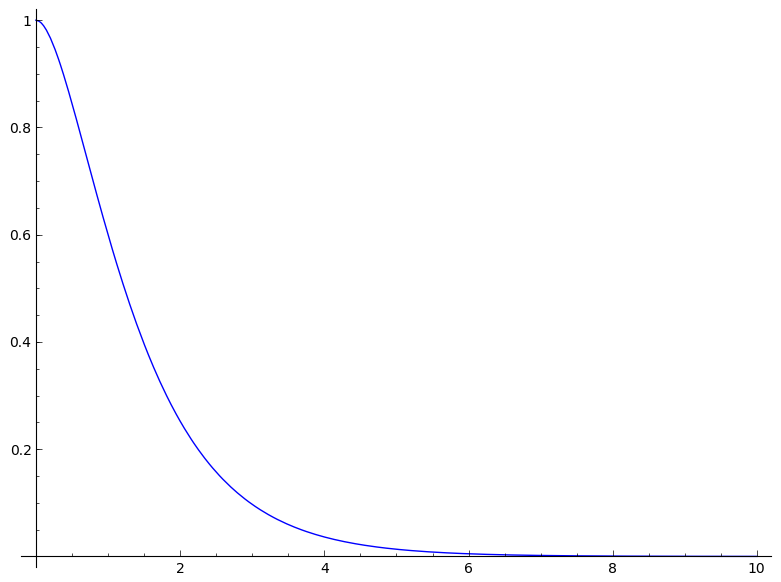
\includegraphics[scale=.2]{imagenes/sobreamortiguado.png}
\caption{ Vibraciones amortiguadas no forzadas ($c>0$, $F=0$) }\label{fig:VibrAmorNoFor}
\end{center}
\end{figure}



\begin{figure}[h]
\begin{center}
\animategraphics[controls, scale=.4]{15}{res_sobre/res_sobre-}{0}{60}
\vspace{.5cm}
\caption{Masa-resorte sobreamortiguado}\label{ani:VibrAmorNoFor}
\end{center}
\end{figure}

Como se observa en la gráfica \ref{fig:VibrAmorNoFor} y la animación \ref{ani:VibrAmorNoFor}
la masa ejecuta una oscilación, lo cual le demanda un tiempo infinito. Podría
haber pasado por la posición de equilibrio sólo en el pasado,
puesto que $x(t)=0$ cuando
\[\boxed{t=\frac{1}{\lambda_1-\lambda_2}\ln\frac{\lambda_1}{\lambda_2}<0}\]


\noindent\textbf{Caso $\Delta=0$.} En esta situación se dice que hay amortiguación crítica. Las raíces son iguales $\lambda_1=\lambda_2=-\mu$. Sabemos que
\boxedeq{x_1(t)=c_1e^{-\mu t}+c_2te^{-\mu t}=e^{-\mu t}\{c_1+c_2t\}}{eq:sol_gen_crit}
Nuevamente la solución puede pasar a lo sumo una vez por la posición de equilibrio, siempre y cuando
$C_2\neq 0$. El compportamiento cualitativo de la solución es muy parecido al caso anterior.


\noindent\textbf{Caso $\Delta<0$, caso subamortiguado.} $\lambda_{1,2}=-\mu\pm\nu i$ con $\nu=\sqrt{|\Delta|}=\sqrt{|\omega^2-\mu^2|}$.
La solución general viene dada por
\boxedeq{x(t)=e^{-\mu t}\left\{ c_1\cos \nu t+c_2\sen \nu t \right\}}{eq:sol_gen_sub}
Está función tiene por gráfica una onda sinusoidal modulada por una función exponencial
decreciente.

\begin{lstlisting}
>>> c1,c2,mu,nu,x0,t=symbols('c1,c2,mu,nu,x0,t')
>>> x=exp(-mu*t)*(c1*cos(nu*t)+c2*sin(nu*t))
>>> C=solve([x.subs(t,0)-x0,x.diff(t).subs(t,0)],[c1,c2])
>>> x=x.subs(C).subs({mu:.1,nu:4,x0:1})
>>> plot(x,(t,0,100))
\end{lstlisting}
\begin{center}
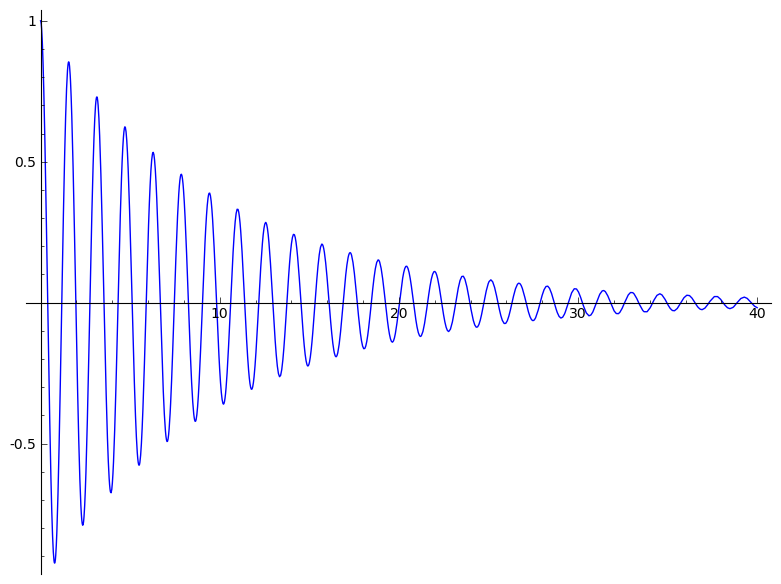
\includegraphics[scale=.15]{imagenes/subamortiguado.png}
\end{center}

{ Vibraciones amortiguadas no forzadas ($c>0$, $F=0$) }
\begin{figure}[h]
\begin{center}
\animategraphics[controls, scale=.4]{15}{res_sub/res_sub-}{0}{60}
%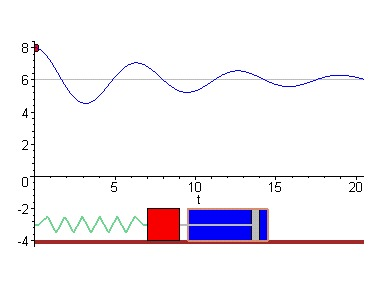
\includegraphics[scale=.4]{res_sub/res_sub-0.jpg}
\vspace{.5cm}
\caption{Masa-resorte subamortiguado}
\end{center}
\end{figure}

Se suele escribir la ecuación \eqref{eq:sol_gen_sub} de otra forma. Expresemos el vector $(c_1,c_2)$ en
coordenadas polares.
\[
c_1=\rho\cos\alpha,\quad c_2=\rho\sen\alpha.
\]
Entonces usando las
\href{https://es.wikipedia.org/wiki/Identidades_trigonom%C3%A9tricas}{fórmulas de adición}
de las funciones trigonométricas
\[
x(t)=e^{-\mu t}\left\{ c_1\cos \nu t+c_2\sen \nu t \right\}=\boxed{\rho e^{-\mu t}\cos(\nu t-\alpha)}.
\]
Llamaremos este régimen \emph{movimiento cuasi-oscilatorio}. Se ejecutan vibraciones, que se disipan con el tiempo,
de \href{http://es.wikipedia.org/wiki/Frecuencia}{frecuencia}
\[
f=\frac{1}{\text{período}}=\frac{\nu}{2\pi},\quad \nu=\sqrt{\omega^2-\mu^2}=\sqrt{\left(\frac{k}{m}\right)^2-
\left(\frac{c}{2m}\right)^2}.
\]
En lugar de la frecuencia se suele considerar la
\href{http://luz.izt.uam.mx/mediawiki/index.php/Frecuencia_angular}{frecuencia angular} que se define como
$2\pi f$. La ventaja de esta definición es que la frecuencia ángular de la función de arriba es
$\nu$.


\noindent\textbf{Ejercicio:} Demostrar que en cualquiera de las situaciones descriptas, $x(t)\to 0$ y $x'(t)\to 0$, cuando $t\to\infty$.
Es decir, el movimiento se va deteniendo.


\subsubsection{ Vibraciones no amortiguadas y forzadas ($\b{c=0}$, $\b{F\neq 0}$) }
Vamos a considerar una fuerza externa oscilatoria de frecuencia angular $\omega_0$ y amplitud $F_0$. Tenemos que resolver
\boxedeq{x''(t)+\omega^2 x(t)=F_0\cos(\omega_0 t).}{eq:ecua_2orden_nohom}
Usaremos el método de coeficientes indeterminados.  Recordar que si $\omega=\omega_0$ estamos en
resonancia. Tendremos que considerar ese caso por separado. Supongamos pues $\omega\neq\omega_0$.
Tenemos que  reemplazar en la ecuación
\[x(t)=A\cos(\omega_0 t)+B\sen(\omega_0 t),\]
y hallar $A$ y $B$ que logren que $x(t)$ sea solución. Usamos SymPy

\begin{lstlisting}
>>> from sympy import *
>>> init_printing()
>>> t,omega,omega0,F0,A,B=symbols('t,omega,omega0,F0,A,B')
>>> x=A*cos(omega0*t)+B*sin(omega0*t)
>>> eq=x.diff(t,2)+omega**2*x-F0*cos(omega0*t)
>>> eqL1=eq.factor().coeff(sin(omega0*t))
>>> eqL2=eq.factor().coeff(cos(omega0*t))
>>> Incog=[A,B]
>>> Ecuas=[eqL1,eqL2]
>>> Matrix([[ecu.coeff(inco) for inco in Incog] for ecu in Ecuas])

\end{lstlisting}
La matríz de coeficientes del sistema de ecuaciones para $A$ y $B$ es
\[\left[\begin{matrix}0 & \omega^{2} - \omega_{0}^{2}\\\omega^{2} - \omega_{0}^{2} & 0\end{matrix}\right]\]
claramente es una matríz no singular, cuando $\omega\neq \omega_0$, y por consiguiente  en no resonancia
tiene una solución
\begin{lstlisting}
>>> SolAB=solve([eqL1,eqL2],[A,B])
>>> x=x.subs(SolAB)
>>> x
\end{lstlisting}

\[x(t)=\frac{F_{0} \cos{\left (\omega_{0} t \right )}}{\omega^{2} - \omega_{0}^{2}}.
\]
La solución general del problema es la solución particular que acabamos de obtener más una solución
general del homogéneo que sabemos es una combinación lineal generica entre $\cos \omega t$ y $\sin \omega t$.

\boxedeq{x(t)=\frac{F_{0} \cos\left(\omega_{0} t\right)}{\omega^{2} - \omega_{0}^{2}}+
c_1\cos(\omega t)+c_2\sin(\omega t).}{eq:sol_gen_noamort_forz}
Como ya hemos visto, considerando las coordenadas polares $\rho$ y $\alpha$ de $c_1,c_2$
podemos reescribir la solución
\[x(t)=\frac{F_{0} \cos\left(\omega_{0} t\right)}{\omega^{2} - \omega_{0}^{2}}+
\rho\cos(\omega t-\alpha)
\]
Vemos que el movimiento es la superposición de dos movimientos oscilatorios de frecuencias $\omega$, que se
denomina la \emph{frecuencia natural} del resorte, y $\omega_0$ que se denomina \emph{frecuencia impresa}.




Resolvamos el pvi
\[
\left\{\begin{array}{l}
x''(t)+\omega^2x(t)=F_0\cos(\omega_0 t),\\
x'(0)=x(0)=0\\
\end{array}
\right.
\]

\begin{lstlisting}
>>> from sympy import *
>>> init_printing()
>>> var('t,c1,c2,omega,omega0,F0')
>>> x=F0/(omega**2-omega0**2)*cos(omega0*t)+c1*cos(omega*t)+c2*sin(omega*t)
>>> C=solve([x.subs(t,0),x.diff(t).subs(t,0)],[c1,c2])
>>> x=x.subs(C)
>>> x
\end{lstlisting}

\[x(t)=-\frac{F_{0} \cos\left(\omega t\right)}{\omega^{2} - \omega_{0}^{2}} + \frac{F_{0} \cos\left(\omega_{0} t\right)}{\omega^{2} - \omega_{0}^{2}}
\]

Ahora usemos la identidad $\cos(a-b)-\cos(a+b)=2\sen a\sen b$, con $a=\frac12 (\omega+\omega_0)$ y
$b=\frac12 (\omega-\omega_0)$. Deducimos
\boxedeq{%
x(t)=\frac{2F_{0} }{\omega^{2} - \omega_{0}^{2}}\sen\left( \frac{\omega-\omega_0}{2}t \right)\sen
\left(\frac{\omega+\omega_0}{2}t\right).
}{eq:sol_gen_pulsos}
Esta expresión la podemos ver como una onda de frecuencia grande $\omega+\omega_0$ modulada por una de frecuencia
chica $\omega-\omega_0$.

\begin{lstlisting}
x=x.subs({F0:1,omega:1,omega0:.9})
plot(x,(t,0,200))
\end{lstlisting}

\begin{figure}[h]
\begin{center}
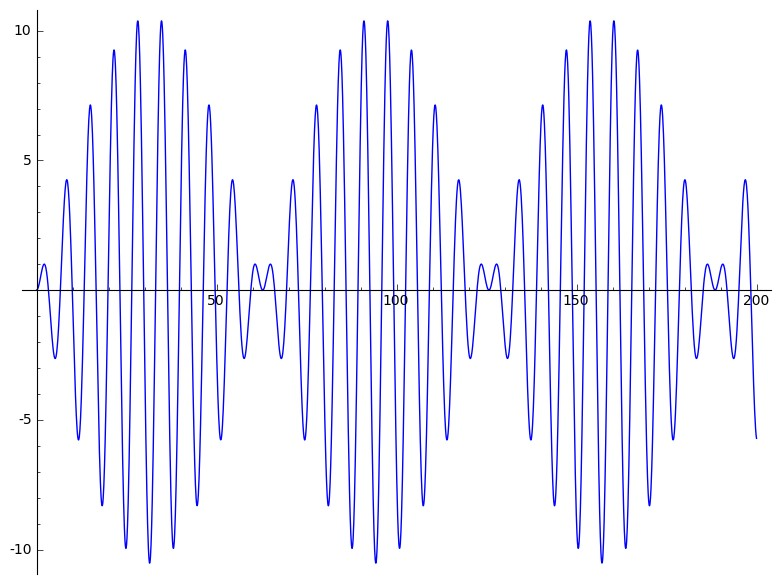
\includegraphics[scale=.15]{imagenes/batido.jpg}
\end{center}
\caption{Fenómeno de batido}\label{fig:batido}
\end{figure}


Calculemos el límite $\lim_{\omega_0\to\omega}x(t)$,

\begin{lstlisting}
>>> limit(x0,omega0,omega)
\end{lstlisting}

\[x(t)=\frac{F_{0} t \sin\left(\omega t\right)}{2 \, \omega}
\]
El caso $\omega=\omega_0$ es el caso con resonancia, que debemos resolver, como fue indicado, proponiendo como solución $y(x)=x\left(A\cos x+ B\sen x\right)$. El siguiente código \texttt{SymPy} muestra que la solución es la misma función
que la obtenida por el proceso de límite de los casos sin resonancia.

\begin{lstlisting}
>>> var('t,omega,F0,A,B')
>>> x=t*(A*cos(omega*t)+B*sin(omega*t))
>>> eq=x.diff(t,2)+omega**2*x-F0*cos(omega*t)
>>> eqL1=eq.factor().coeff(sin(omega*t))
>>> eqL2=eq.factor().coeff(cos(omega*t))
>>> SolAB=solve([eqL1,eqL2],[A,B])
>>> x=x.subs(SolAB)
\end{lstlisting}



Se producen ``vibraciones'' no acotadas.
\begin{lstlisting}
>>> plot(x.subs({omega:1,F0:1}),(t,0,100))
\end{lstlisting}

\begin{figure}[h]
\begin{center}
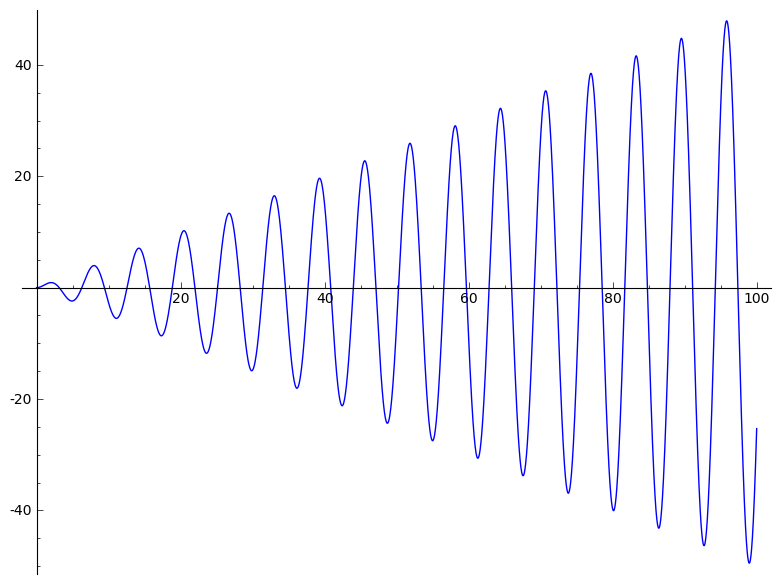
\includegraphics[scale=0.3]{imagenes/osc_arm_forz_res.png}
\end{center}
\caption{Resonancia}
\end{figure}
En la wiki \href{http://wiki.sagemath.org/interact/misc\#Hearing_a_trigonometric_identity}{Hearing a trigonometric identity}
se puede escuchar ondas sonoras con los fenómenos de resonancia y batido.

\subsubsection{Vibraciones amortiguadas y forzadas ($\b{c>0}$, $\b{F\neq 0}$) }
Vamos a considerar una fuerza externa oscilatoria de frecuencia $\omega_0$ y amplitud $F_0$. Tenemos que resolver
\boxedeq{x''(t)+2\mu x'(t)+\omega^2 x(t)=F_0\cos(\omega_0 t).}{eq:ecua_2orden_amort_nohom}
Proponemos por solución $x(t)=A\cos(\omega_0 t)+B\sen(\omega_0 t)$.

\begin{lstlisting}
>>> var('t,mu,omega,omega0,F0,A,B')
>>> x=A*cos(omega0*t)+B*sin(omega0*t)
>>> eq=x.diff(t,2)+2*mu*x.diff(t)+omega**2*x-F0*cos(omega0*t)
>>> eqL1=eq.factor().coeff(sin(omega0*t))
>>> eqL2=eq.factor().coeff(cos(omega0*t))
>>> Incog=[A,B]
>>> Ecuas=[eqL1,eqL2]
>>> M=Matrix([[ecu.coeff(inco) for inco in Incog] for ecu in Ecuas])
>>> M.det()
\end{lstlisting}

La matríz $M$ del sistema lineal que satisfacen las incognitas $A$ y $B$ tiene determninante
\[\det(M)=- 4 \mu^{2} \omega_{0}^{2} - \omega^{4} + 2 \omega^{2} \omega_{0}^{2} - \omega_{0}^{4}.
\]
No queda claro si, eventualmente, puede ser singular. Calculando las posibles soluciones para $\omega$ de $\det(M)=0$
\begin{lstlisting}
>>> solve(M.det(),omega)
\end{lstlisting}
\[\left [ - \sqrt{- 2 i \mu \omega_{0} + \omega_{0}^{2}}, \quad \sqrt{- 2 i \mu \omega_{0} + \omega_{0}^{2}}, \quad - \sqrt{2 i \mu \omega_{0} + \omega_{0}^{2}}, \quad \sqrt{2 i \mu \omega_{0} + \omega_{0}^{2}}\right ]
\]
son todas complejas no reales, por consiguiente la matríz es simpre no singular.
\begin{lstlisting}
>>> SolAB=solve([eqL1,eqL2],[A,B])
>>> x.subs(SolAB)
\end{lstlisting}

\boxedeq{x(t)= \frac{2 F_{0} \mu \omega_{0} \sin{\left (\omega_{0} t \right )}}{4 \mu^{2} \omega_{0}^{2} + \left(\omega^{2} - \omega_{0}^{2}\right)^{2}} + \frac{F_{0} \left(\omega^{2} - \omega_{0}^{2}\right) \cos{\left (\omega_{0} t \right )}}{4 \mu^{2} \omega_{0}^{2} + \left(\omega^{2} - \omega_{0}^{2}\right)^{2}}
}{eq:SolGennoHom}
Es un movimiento oscilatorio de frecuencia angular $\omega_0$. Podemos escribir $x(t)=\rho\cos(\omega_0 t-\alpha)$,
donde $(\rho,\alpha)$ son las coordenadas polares de $(A,B)$. En particular la amplitud de la oscilación viene dada por  $\rho=\sqrt{A^2+B^2}$.
Recurrimos nuevamente a SymPy para calcular $\rho$.

\begin{lstlisting}
>>> rho=sqrt(A**2+B**2).subs(SolAB).simplify()
>>> rho
\end{lstlisting}
\[
\rho(\omega_0)=
\frac{F_{0}}{\sqrt{(\omega^2-\omega_0^2)^2+4\mu^2\omega_0^2}}
\]
%
% \[\alpha=\atan2\left( {{\omega^{2} -
% \omega_{0}^{2}} } , {2 \, \mu \omega_{0} } \right)
% \]
%En una consola de sage entrar \texttt{atan2?} para averiguar que función es $\atan2$.
Grafiquemos la función $\rho(\omega_0)$ para $\omega=5$ y $\mu=0.1$.
\begin{lstlisting}
>>> plot(rho.subs({F0:1, mu:.1,omega:5}),(omega0,0,10))
\end{lstlisting}
\begin{figure}[h]
\begin{center}
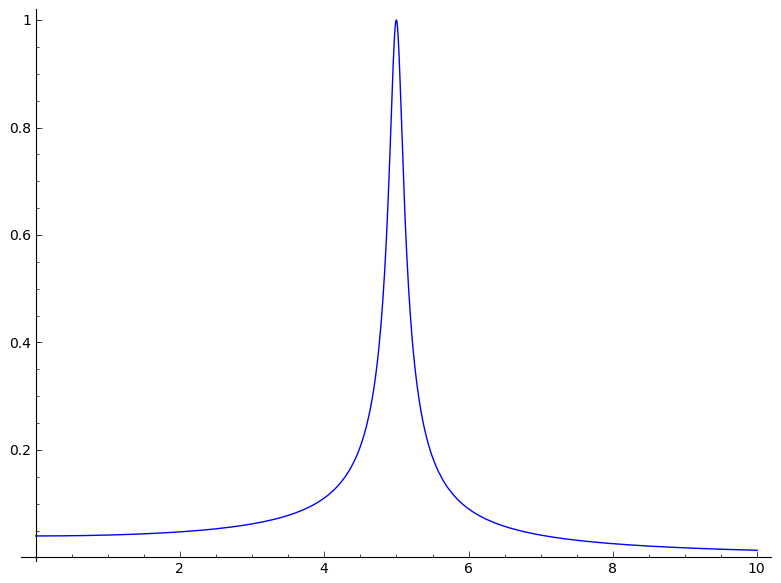
\includegraphics[scale=.3]{imagenes/rho_graf.png}
\end{center}
\caption{Gráfico amplitud vs. frecuencia, resorte amortiguado y forzado}
\end{figure}
La función tiene un notorio máximo cerca de $\omega_0=5$. Seguramente es debido a la aparición de resonancias. Hallemos el punto de máximo exacto, primero encontremos puntos críticos.
\begin{lstlisting}
>>> sol=solve(rho.diff(omega0),omega0)
>>>sol
\end{lstlisting}
\[\left [ 0, \quad - \sqrt{- 2 \mu^{2} + \omega^{2}}, \quad \sqrt{- 2 \mu^{2} + \omega^{2}}, \quad - \sqrt{\tilde{\infty} \sqrt{F_{0}^{2}} - 2 \mu^{2} + \omega^{2}}, \quad \sqrt{\tilde{\infty} \sqrt{F_{0}^{2}} - 2 \mu^{2} + \omega^{2}}\right ]
\]
El único lícito, si $2\mu^2<\omega$,  es $\hat{\omega}_0=\sqrt{- 2 \mu^{2} + \omega^{2}}$.  Podemos constatar el caracter,  si es máximo/mínimo o ninguna de estas opciones. Calculando la derivada segunda
\begin{lstlisting}
>>> rho.diff(omega0,2).subs(omega0,sol[2])
\end{lstlisting}
\[
\frac{2 \sqrt{\frac{F_{0}^{2}}{4 \mu^{4} + 4 \mu^{2} \left(- 2 \mu^{2} + \omega^{2}\right)}} \left(4 \mu^{2} - 2 \omega^{2}\right)}{4 \mu^{4} + 4 \mu^{2} \left(- 2 \mu^{2} + \omega^{2}\right)}
\]
vemos que es claramente negativa. Luego tenemos un máximo local en $\hat{\omega}_0$. Comparando el valor de $\rho(\hat{\omega}_0)$ con los de $\rho(0)$ y $\rho(+\infty)$ determinamos si es máximo global. Un cálculo, que podemos hacer con SymPy, nos muestra que
\[\lim_{\omega_0\to\infty}\rho(\omega_0)=0<\frac{F_0}{\omega^2}=\rho(0)< \frac12\frac{F_0}{\mu\sqrt{\omega^2-\mu^2}}=\rho(\hat{\omega}_0).\]
En consecuencia $\hat{\omega}_0$ es máximo absoluto.



En el ejemplo que graficamos
el máximo ocurre en
\begin{lstlisting}
>>> sol[2].subs({mu:.1,omega:5})
4.99799959983992
\end{lstlisting}

Vale decir, un oscilador armónico en reposo es más sensible a excitaciones en ciertas frecuencias, aproximadamente igual a la frecuencia
natural del resorte cuando el coeficiente de viscocidad $c=2m\mu$ es chico. Esto es utilizado para diseñar dispositivos que captan ondas sísmicas.


Hasta aquí hemos encontrado una solución particular del sistema no homogéneo. Para encontrar una solución general deberíamos adicionar a la particular que disponemos
una solución general $x_g(t)$ de la ecuación homogénea. La forma de esta solución general es de alguno de los tipos \ref{eq:sol_gen_sub},
\ref{eq:sol_gen_crit} o \ref{eq:sol_sub_amor}. Sin embargo no nos importa ahora la fórmula explícita de estas soluciones, sino que nos interesa resaltar que
trátese del tipo que se trate, se satisface que $\lim_{t\to\infty}x_g(t)=0$. Por este motivo, vamos a decir que esta parte de la solución es
\emph{transitoria}. En cambio la solución que prevalece en el tiempo dada por \eqref{eq:SolGennoHom} la denominaremos solución \emph{estacionaria}.

\subsection{Un poco de mecánica celeste}

Vamos a considerar ahora el problema del movimiento de un planeta, digamos la Tierra, de masa $m_{\earth}$ alrededor del sol, de masa $m_{\sun}$. Como
$m_{\sun}\gg m_{\earth}$ vamos a ignorar la fuerza que actúa sobre el Sol debido a la atracción gravitatoria de la Tierra. Esta suposición, aunque falsa, la hacemos
por simplicidad. No obstante, con sólo un poco de trabajo, el caso más general se reduce al tratado aquí. Ver el \href{https://drive.google.com/file/d/0B80iJ0HgObRRbUtUQ2hFQ0FlTG8/view}{trabajo final} de la Lic. Matemática de Leopoldo Buri,
para una deducción más cuidadosa. Vamos a suponer además que el movimiento del planeta se retringe a un plano. Esta afirmación es cierta y aunque su demostración
es sencilla no la desarrollaremos aquí.
Supongamos un sistema de coordenadas cartesianas sobre el plano en que se realiza el movimiento orbital del planeta. Asumimos el Sol en el origen de coordenadas y en
reposo. Como no actúa fuerza sobre él, permanecerá en esa situación. Vamos a suponer que la posición de la Tierra es $\vec{r}$.

Los dos ingredientes básicos para derivar la leyes de movimiento del planeta son la
\href{http://es.wikipedia.org/wiki/Leyes_de_Newton\#Segunda_ley_de_Newton_o_ley_de_fuerza}{Segunda Ley de Newton} y la
\href{http://es.wikipedia.org/wiki/Ley_de_gravitación_universal}{Ley Gravitación Universal}. Ya hemos considerado ambas con anterioridad.
Según la Ley de Gravitación Universal, la magnitud de la fuerza de gravedad es proporcional a $\frac{m_{\earth}m_{\sun}}{d^2}$, donde $d$ es la distancia tierra-sol.
A la constante de proporcionalidad la llamaremos, como es costumbre, $G$. La dirección de la fuerza gravitatoria es la de la recta que une los dos astros y
el sentido es tal que la fuerza es atractiva entre los cuerpos. Vale decir, la dirección y sentido de la
fuerza de gravedad vienen dados por el versor $-\vec{r}/r$, donde $r=|\vec{r}|$. Luego se debe satisfacer que
\[m_{\earth}\frac{d^2\vec{r}}{dt^2}=-\frac{Gm_{\earth}m_{\sun}}{r^2}\frac{\vec{r}}{r}=-Gm_{\earth}m_{\sun}\frac{\vec{r}}{r^3}. \]


Es decir
\boxedeq{\frac{d^2\vec{r}}{dt^2}=-\mu\frac{\vec{r}}{r^3}\quad\text{donde } \mu:=Gm_{\sun}}{eq:grav}
Esta ecuación se conoce como la \href{http://es.wikipedia.org/wiki/Problema_de_los_dos_cuerpos}{ecuación de los dos cuerpos}.
Dado que esta ecuación entraña, a su vez, tres ecuaciones escalares, una por cada
componente de $\vec{r}$, se nos presenta aquí un \emph{Sistema de Ecuaciones Diferenciales}. No sabemos resolver sistemas de ecuaciones. No obstante vamos
a ver como podemos reducir la ecuación anterior, mediante ingeniosos cambios de
variables, a ecuaciones diferenciales que sabemos resolver.


Vamos a usar coordenadas polares $(r,\theta)$ y los versores $\vec{u}_r:=(\cos\theta,\sen\theta)$ y $\vec{u}_{\theta}:=(-\sen\theta, \cos\theta)$. Notar que
$\vec{u}_r \perp \vec{u}_{\theta}$ y por consiguiente $\mathcal{B}:=\{\vec{u}_r , \vec{u}_{\theta}\}$ forma una base del espacio euclideano 2-dimensional. Usaremos este hecho
para representar distintos vectores como combinación lineal de vectores de la base. Los cálculos, como es ya habitual, se los dejaremos a SymPy,


Primero declaramos las variables y asignamos los vectores $\vec{u}_r$, $\vec{u}_{\theta}$ y el vector
$\vec{r}$ al que llamamos \texttt{pos}.

\begin{lstlisting}
>>> from sympy import *
>>> init_printing()
>>> var('t,mu')
>>> x,y,r,theta=symbols('x,y,r,theta',cls=Function)
>>> u_r=Matrix([cos(theta(t)),sin(theta(t))])
>>> u_theta=Matrix([-sin(theta(t)),cos(theta(t))])
>>> pos=r(t)*u_r
\end{lstlisting}



Como vamos a necesitar representar vectores en la base $\mathcal{B}=\{\vec{u}_r , \vec{u}_{\theta}\}$, construímos una matriz
con los vectores de la base en las columnas.
\begin{lstlisting}
>>> M=u_r.row_join(u_theta)
\end{lstlisting}
Concretamente queremos representar el vector aceleración $\vec{a}:=\tfrac{d^2\vec{r}}{dt^2}$ en la base $\mathcal{B}$, para ello debemos resolver $MX=\vec{a}$, donde $X$ y
$\vec{a}$ los asumimos vectores columna. Con SymPy lo hacemos en un periquete

\begin{codigo}[\texttt{linsolve}]
Resuelve un sistema $Ax=b$

\textbf{Sintaxis} (\href{http://docs.sympy.org/dev/modules/solvers/solveset.html#sympy.solvers.solveset.linsolve}{documentación \texttt{SymPy}})

\texttt{linsolve((A,b), símbolos)}

\texttt{(A,b):} tuple con la matríz y el término independientre del sistema.

\texttt{símbolos:} Muchas veces la solución no es única, en ese caso trata de representar la solución paramétricamente con los símbolos introducidos por \texttt{símbolos}.

\texttt{Retorna: } Un conjunto finito (tipo de datos de SymPy).

\end{codigo}



\begin{lstlisting}
>>> alpha=symbols('alpha')
>>> a=linsolve((M,pos.diff(t,2)),alpha )
>>> a=list(a) #convertimos de finite set a list
>>> a=a[0] #es una lista de tuples, sacamos el tuple
>>> a
\end{lstlisting}

\[
 \left\{\left ( - r{\left (t \right )} \frac{d}{d t} \theta{\left (t \right )}^{2} + \frac{d^{2}}{d t^{2}}  r{\left (t \right )}, \quad r{\left (t \right )} \frac{d^{2}}{d t^{2}}  \theta{\left (t \right )} + 2 \frac{d}{d t} r{\left (t \right )} \frac{d}{d t} \theta{\left (t \right )}\right )\right\}
\]
Obtenemos asi las dos componetes de $\vec{a}$.
\[
\vec{a}=\left(\begin{array}{c}
\ddot{r}-r\dot{\theta}^2 \\
r\ddot{\theta}+2\dot{r}\dot{\theta}
\end{array}
\right)=
\left(\begin{array}{c}
\ddot{r}-r\dot{\theta}^2 \\
\frac{1}{r}\frac{d}{dt} \left( r^2\dot{\theta} \right)
\end{array}
\right)
\]


El vector aceleración debe ser igual a la fuerza por unidad de masa $-\mu \vec{r}/r^3$. Notemos que esta fuerza es
\href{http://es.wikipedia.org/wiki/Campo_central}{central}, es decir tiene componente nula
respecto al vector $\vec{u}_{\theta}$. Por consiguiente se debe satisfacer que
\[\frac{1}{r}\frac{d}{dt} \left( r^2\dot{\theta} \right)=0\Longleftrightarrow \exists h\in\mathbb{R}: \boxed{ r^2\dot{\theta}=h}. \]




\begin{wrapfigure}[12]{l}{5cm}
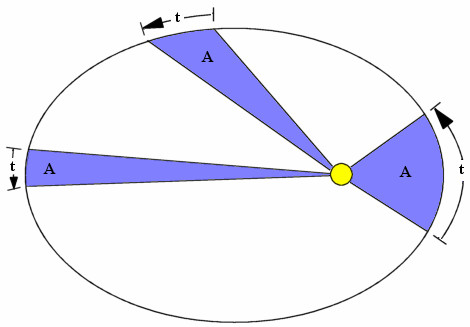
\includegraphics[scale=.3]{imagenes/2leykepler.jpeg}\\
\end{wrapfigure}
Hemos derivado la \href{http://es.wikipedia.org/wiki/Leyes_de_Kepler}{Segunda Ley de Kepler}: El radio vector barre áreas iguales en tiempos iguales.



En la dirección radial $\vec{u}_r$ la componente de la fuerza es $-\mu/r^2$. Es decir se satisface la ecuación
\[
\ddot{r}-r\dot{\theta}^2=-\frac{\mu}{r^2}
\]
Notar que esta ecuación entraña dos incognitas $r$ y $\theta$, pero $\dot{\theta}$ puede ser remplazado por $h/r^2$ por la segunda Ley de Kepler.
Declaremos la variable $h$ que juega un rol importante y reemplacemos $\dot{\theta}$ en la ecuación

\begin{lstlisting}
>>> var('h')
>>> ed=(a[0]).subs((theta(t)).diff(t),h/r(t)**2)
>>> ed+=mu/r(t)**2
\end{lstlisting}
Resulta
\[- \frac{h^{2}}{r^{3}{\left (t \right )}} + \frac{\mu}{r^{2}{\left (t \right )}} + \frac{d^{2}}{d t^{2}}  r{\left (t \right )}=0.
\]
Conseguimos una ecuación no lineal de segundo orden para $r$. De los métodos que hemos visto, ninguno se aplica a esta ecuación.
El truco mágico consiste en considerar la nueva variable dependiente $z=1/r$ y la nueva variable independiente
$\theta$.

\begin{lstlisting}
>>> z=Function('z')(theta(t))
>>> r=1/z
>>> ed2=r.diff(t,2)+mu/r**2-h**2/r**3
>>> ed2
\end{lstlisting}
Se obtiene
\[
\begin{split}
 0&=- h^{2} z^{3}{\left (\theta{\left (t \right )} \right )} + \mu z^{2}{\left (\theta{\left (t \right )} \right )} + \frac{1}{z^{2}{\left (\theta{\left (t \right )} \right )}} \left(- \frac{d}{d t} \theta{\left (t \right )}^{2} \frac{d^{2}}{d \theta{\left (t \right )}^{2}}  z{\left (\theta{\left (t \right )} \right )}\right.\\
 &\quad\left.- \frac{d^{2}}{d t^{2}}  \theta{\left (t \right )} \left. \frac{d}{d \xi_{1}} z{\left (\xi_{1} \right )} \right|_{\substack{ \xi_{1}=\theta{\left (t \right )} }}+ \frac{2 \frac{d}{d t} \theta{\left (t \right )}^{2}}{z{\left (\theta{\left (t \right )} \right )}} \left. \frac{d}{d \xi_{1}} z{\left (\xi_{1} \right )} \right|_{\substack{ \xi_{1}=\theta{\left (t \right )} }}^{2}\right)
\end{split}
\]
En la complicada ecuación resultante nuevamente aparece $\theta'$ y además ahora aparece $\theta''$. Tenemos que reemplazar
$\theta'$ por $hz^2$ y $\theta'$ por $\tfrac{d}{dt}hz^2$.
\begin{lstlisting}
>>> theta2diff=(h*z**2).diff(t).subs(theta(t).diff(t),h*z**2)
>>> ed3=ed2.subs({theta(t).diff(t):h*z**2,theta(t).diff(t,2):theta2diff})
>>> ed4=(ed3/z**2/h**2).expand()
>>> ed4
\end{lstlisting}
Resulta
\[- z{\left (\theta{\left (t \right )} \right )} - \frac{d^{2}}{d \theta{\left (t \right )}^{2}}  z{\left (\theta{\left (t \right )} \right )} + \frac{\mu}{h^{2}}=0.
\]
La ecuación del oscilador armónico. Sabemos resolver esta ecuación y S también!!
\begin{lstlisting}
>>> var('theta')
>>> z=Function('z')(theta)
>>> ed5=ed4.subs(theta(t),theta)
>>> dsolve(ed5,z).simplify()
\end{lstlisting}
Obtenemos
\[
z{\left (\theta \right )} = C_{1} \sin{\left (\theta \right )} + C_{2} \cos{\left (\theta \right )} + \frac{\mu}{h^{2}}.
\]
Ahora si escribimos $C_1=\rho\cos\omega$ y $C_2=-\rho\sen\omega$ y recordamos que $z=1/r$, deducimos
\[r=\frac{1}{\frac{\mu}{h^2}+\rho\sen(\theta-\omega)}\]
Llamando $p=\tfrac{h^2}{\mu}$ y $e=\tfrac{\rho h^2}{\mu}$
\boxedeq{r=\frac{p}{1+e\sen(\theta-\omega)}}{eq:orb_elipse}

\noindent\textbf{Ejercicio:} La ecuación \eqref{eq:orb_elipse} es la ecuación de una cónica con foco en el origen y excentricidad $e$.
Recordemos que la variable $\theta$ es el ángulo polar. Hagamos algunos gráficos para distintas excentricidades.
\begin{lstlisting}
from sympy.plotting import plot_parametric
""" Gráfico de excentricidades menores a uno  """
cant=20
e_s=[.04*j for j in range(cant)]
e=e_s[0]
p=plot_parametric(1/(1+e*cos(theta))*cos(theta),\
                  1/(1+e*cos(theta))*sin(theta),\
                  (theta,0,6.28),show=False)


for e in e_s[1:]:
    p1=plot_parametric(1/(1+e*cos(theta))*cos(theta),\
                       1/(1+e*cos(theta))*sin(theta),\
                       (theta,0,6.28),show=False)
    p.append(p1[0])

""" Gráfico de excentricidades mayores a uno  """
e_s=[.04*j+1 for j in range(1,cant)]
for e in e_s:
    p1=plot_parametric(1/(1+e*cos(theta))*cos(theta),\
                       1/(1+e*cos(theta))*sin(theta),\
                       (theta,-pi*2/3,pi*2/3),show=False,line_color=(0,1,0))
    p.append(p1[0])

p.show()
\end{lstlisting}

\begin{center}
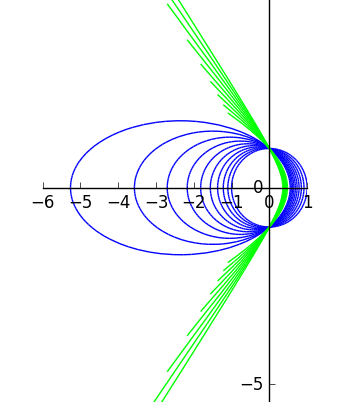
\includegraphics[scale=.5]{imagenes/conicas.png}
\end{center}


Hemos logrado encontrar $r$ como función de $\theta$. No obstante
no hemos logrado resolver aún el problema de los dos cuerpos \eqref{eq:grav}, para ello deberíamos encontrar $\vec{r}(t)$, es decir poner a $
\vec{r}$ como función de $t$. Esto nos serviría para decir que punto de la órbita ocupa el planeta en un dado momento. Este problema no lo desarrollaremos aquí dado
que su solución se aparta del tema de las ecuaciones diferenciales.


\section{Ecuaciones lineales de orden superior}


\begin{definicion}[Ecuación lineal general de orden $n$]{}
Es una ecuación de la forma
\boxedeq{y^{(n)}(x)+p_{n-1}(x)y^{(n-1)}(x)+\cdots+p_0(x)y(x)=r(x)}{eq:ecua_lin_gen_orden_n}
donde $p_i,r$, $i=0,\ldots,n-1$ son funciones definidas en un intervalo $I$
\end{definicion}


Los resultados y técnicas que hemos desarollado para ecuaciones de orden $2$ se aplican con cambios previsibles a ecuaciones de mayor orden. Exponemos de manera sumaria
estos resultados.

\subsection{Existencia y unicidad de soluciones}

\begin{teorema}[Teorema de existencia y unicidad de soluciones]{}
 Supongamos $p_i,r$, $i=0,\ldots,n-1$ continuas sobre $I$. Sean $x_0\in I$ e $y_0,y_1,\ldots y_{n-1}\in\rr$ dados. Entonces existe una única solución del PVI
 \[\left\{
 \begin{array}{l l l}
   y^{(n)}(x)+&p_{n-1}(x)y^{(n-1)}(x)+\cdots+p_0(x)y(x)=r(x),x\in I\\
   y(x_0)&=y_0&\\
   y'(x_0)&=y_1&\\
   &\vdots\\
  y^{(n-1)}(x_0)&=y_{n-1}&\\
  \end{array}\right.
\]

\end{teorema}


\subsection{Estructura del conjunto de soluciones}

\begin{teorema}[Estructura conjunto de soluciones ecuaciones homogéneas]{}
Supongamos $y_1,y_2,\ldots,y_n$ soluciones linealmente independientes de
\[y^{(n)}(x)+p_{n-1}(x)y^{(n-1)}(x)+\cdots+p_0(x)y(x)=0.\]
Entonces
\[y=c_1y_1+\cdots+c_ny_n,\quad c_i\in\rr, i=1,\ldots,n,\]
es solución general. Vale decir, el conjunto de soluciones es un espacio vectorial $n$-dimensional.
\end{teorema}



\begin{teorema}[Estructura conjunto de soluciones ecuaciones no homogéneas]{}
Una solución general de la ecuación no homogénea
\[y^{(n)}(x)+p_{n-1}(x)y^{(n-1)}(x)+\cdots+p_0(x)y(x)=r(x),\]
es la suma de una solución particular de esta ecuación más una solución general de la ecuación homogénea asociada.
\end{teorema}






\begin{teorema}[Fórmula Abel]{}
Si $y_1,y_2,\ldots,y_n$ son soluciONES de la ecuación  homogénea
\boxedeq{y^{(n)}(x)+p_{n-1}(x)y^{(n-1)}(x)+\cdots+p_0(x)y(x)=0,}{eq:lin_hom_orden_n}
Entonces el Wronskiano satisface
\boxedeq{W(y_1,\ldots,y_n)(x)=W(y_1,\ldots,y_n)(x_0)e^{-\int_{x_0}^xp_{n-1}(t)dt}.}{eq:formu_abel}
En particular  $\{y_1,y_2,\ldots,y_n\}$ son linalmente independientes si y solo si $W(x)\neq 0$ para todo $x\in I$.
\end{teorema}

\textbf{Dem.} Las demostraciones de los resultados anteriores es tan similar a su análogo de orden 2 que no vale la pena invertir tiempo en ellas. La demostración de la fórmula de Abel, si nos parece lo suficientemente interesante para dejarla como \textbf{ejercicio}.



\subsection{Ecuaciones homogéneas con coeficientes constantes}
Las ecuaciones lineales de orden $n$, homogeneas con coeficientes constantes  se resuelven por métodos análogos a los considerados para ecuaciones de segundo orden. Se propone $y(x)=e^{rx}$ como solución. Reemplazando esta función
en \eqref{eq:lin_hom_orden_n} vemos que $y$ sería solución si y solo si $r$ es solución de la ecuación característica
\boxedeq{r^n+p_{n-1}r^{n-1}+\cdots+p_1r+p_0=0.}{eq:ecua_carac}
Ahora se presentan diversos casos.



\subsubsection{Raices reales distintas.} Si la ecuación característica \eqref{eq:ecua_carac} tiene $n$ raíces $r_1,\ldots,r_n$ reales y distintas entonces
$y_1(x)=e^{r_1x},\ldots,y_n(x)=e^{r_nx}$ son soluciones linealmente independientes y por ende
\[\boxed{y(x)=c_1e^{r_1x}+\cdots+c_ne^{r_nx}}\]
es solución general.

Dejamos como ejercicio la demostración de la independencia lineal. En lugar de usar el Wronskiano, se puede utilizar  la siguiente idea basada en métodos operacionales. Denotemos por $D$  el operador diferenciación, esto es $D$ es sencillamente la función  definida sobre el conjunto de funciones diferenciables sobre un intervalo abierto y que actúa derivando, esto es $Dy=y'(x)$. Dado un polinomio $p(X)=p_nX^n+p_{n-1}X^{n-1}+\cdots+p_1X+p_0$, $p_i\in\rr$, $i=0,\ldots,n$, denotamos por  $p(D)$ el operador definido por
\[p(D)y=p_ny^{(n)}+p_{n-1}y^{(n-1)}+\cdots+p_1y'+p_0y.\]
Diremos que $p(D)$ es un \emph{operador diferencial polinomial}.

\noindent\textbf{Ejercicio 1} Dado que dos polinomios se pueden sumar y multiplicar, resultando estas operaciones en un nuevo polinomio, es posible hacer lo propio con operadores diferenciales polinomiales. Demostrar que el producto de dos de tales operadores  $p(D)$ y $q(D)$ es conmutativo. Esta propiedad es lo mismo que afirmar que el producto de polinomios es conmutativo. Analizar que ocurriría si permitiésemos que los coeficientes $p_i$ fuesen funciones de $x$, $p_i=p_i(x)$.


\noindent\textbf{Ejercicio 2} Supongamos ahora que $r_1,\ldots,r_n$ son números reales distintos y que
\[y=c_1e^{r_1x}+c_2e^{r_2x}+\cdots+c_ne^{r_nx}.\]
Considerar el operador diferencial
\[p(D)=(D-r_1)\cdots(D-r_{i-1})(D-r_{i+1})\cdots(D-r_n).\]
Demostrar que
\[p(D)y=(r_i-r_1)\cdots(r_i-r_{i-1})(r_i-r_{i+1})\cdots(r_i-r_n)e^{r_ix}.\]
Deducir de esto la independencia lineal de $\{e^{r_1x},\ldots,e^{r_nx}\}$.



\subsubsection{Raices reales repetidas.}
Supongamos que la ecuación característica \eqref{eq:ecua_carac} tiene  raíces reales repetidas. Sean $r_1,\ldots,r_k$ las raices distintas y $m_j$ la multiplicidad de la raíz $r_j$. Por cada raíz $r_j$ considerar las $m_j$  funciones

\[\mathcal{B}_j:=\{y_j^0(x)=e^{r_jx}, y_j^1(x)=xe^{r_jx},\ldots y_j^{m_j-1}(x)=x^{m_j-1}e^{r_jx}\}.\]

 \noindent\textbf{Ejercicio 3} Demostrar que $\mathcal{B}:=\mathcal{B}_1\cup\cdots\cup \mathcal{B}_k$ forma
 un conjunto de  $n$  soluciones linealmente independientes.

\subsubsection{Raices complejas.}
Supongamos que la ecuación característica \eqref{eq:ecua_carac} tiene  raíces complejas. Como la ecuación característica tiene coeficientes reales, las raices aparecen de a pares conjugados $\mu\pm\nu i$. Si las raices son simples por cada uno de estos pares hay que considerar las soluciones
\[e^{\mu x}\cos x\quad\text{y}\quad e^{\mu x}\sen x.\]
Si son múltiples con multiplicidad $k$ hay que considerar las $2k$ soluciones
\[x^0e^{\mu x}\cos x,\ldots, x^{k-1}e^{\mu x}\cos x\quad\text{y}\quad x^0e^{\mu x}\sen x,\ldots x^{k-1}e^{\mu x}\sen x .\]
Dejamos los detalles que es necesario completar como trabajo práctico.




\subsection{Aplicación: osciladores armónicos acoplados}
Supongamos dos masas $m_1$ y $m_2$ sujetas a dos puntos fijos por sendos resortes y, a su vez, unidas entre si por un tercer resorte.
\begin{center}
\animategraphics[controls, scale=.4]{15}{osciladores_acoplados/osci-}{0}{751}
 \end{center}

Vamos a medir la posición de las masas desde origenes distintos situados en los respectivos puntos de equilibrio. Por consiguiente las posiciones $x$ e $y$ de las masas representan también su desplazamiento desde el equilibrio.  Utilizando la segunda ley de Newton, la Ley de Elasticidad de Hooke  y tomando en consideración que el resorte central está desplazado desde su estado de equilibrio en una cantidad igual a $y-x$, vemos que se debe satisfacer que
% \[\left\{ \begin{array}{l l}
%              m_1x''(t)=-k_1x +k_3(y-x)\\
%              m_2y''(t)=-k_3(y-x)-k_2y
%             \end{array} \right.
% \]
\begin{subequations}
\label{eq:tot}
\begin{empheq}[left=\empheqlbrace]{align}
             m_1x''(t)=-k_1x +k_3(y-x)\label{eq:sis1}\\
             m_2y''(t)=-k_3(y-x)-k_2y\label{eq:sis2}
\end{empheq}
\end{subequations}

\begin{center}
  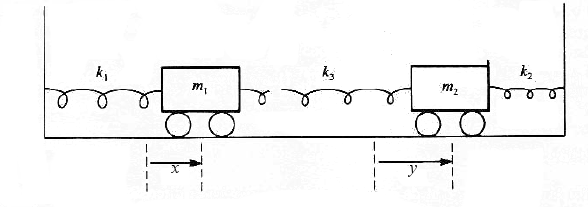
\includegraphics[scale=.4]{imagenes/osci_aco.png}
\end{center}


Se nos presentó un sistema de ecuaciones de segundo orden. Vamos a poder convertirlo en una ecuación pagando el precio de incrementar el orden. El procedimiento es derivar \eqref{eq:sis1} (obviamente es lo mismo empezar por \eqref{eq:sis2}) dos veces respecto a $t$. En el resultado sustituímos $y''$ por su igual según \eqref{eq:sis2}. El resultado es una ecuación que todavía tiene la variable $y$, pero podemos usar \eqref{eq:sis1} para sustituir $y$ por una expresión que sólo tiene $x$ y sus derivadas. Todo esto lo haremos con SymPy.



\begin{lstlisting}
>>> from sympy import *
>>> init_printing()
>>> var('x,y,t,m1,m2,k1,k2,k3')
>>> x,y=symbols('x,y',cls=Function)
>>> eq1=m1*x(t).diff(t,2)+k1*x(t)-k3*(y(t)-x(t))
>>> eq2=m2*y(t).diff(t,2)+k2*y(t)+k3*(y(t)-x(t))
>>> sust1,=solve(eq2,y(t).diff(t,2))
>>> sust2,=solve(eq1,y(t))
>>> eq3=eq1.diff(t,2).subs({y(t).diff(t,2):sust1, y(t):sust2})
>>> eq3.expand().collect(x(t))
\end{lstlisting}
 Obtenemos la ecuación de cuarto orden
\[
\begin{split}
 m_{1} \frac{d^{4}}{d t^{4}} & x{\left (t \right )} + \left(\frac{k_{1} k_{2}}{m_{2}} + \frac{k_{1} k_{3}}{m_{2}} + \frac{k_{2} k_{3}}{m_{2}}\right) x{\left (t \right )}\\ &+ \left(k_{1} + \frac{k_{2} m_{1}}{m_{2}} + \frac{k_{3} m_{1}}{m_{2}} + k_{3}\right) \frac{d^{2}}{d t^{2}}  x{\left (t \right )}=0.
\end{split}
\]
 Vamos a suponer todos los parámetros igual a 1. Encontremos y resolvamos la ecuación característica
 \begin{lstlisting}
>>> eq4=eq3.subs({m1:1,m2:1,k1:1,k2:1,k3:1})
>>> eq4
\end{lstlisting}
\[3 x{\left (t \right )} + 4 \frac{d^{2}}{d t^{2}}  x{\left (t \right )} + \frac{d^{4}}{d t^{4}}  x{\left (t \right )}=0.\]





\begin{lstlisting}
>>> r=var('r')
>>> z=exp(r*t)
>>> eq5=eq4.subs({x(t):z,x(t).diff(t,4):z.diff(t,4),x(t).diff(t,2):z.diff(t,2)})/z
>>> eq5.expand()
\end{lstlisting}
Las soluciones de la ecuación característica son ${sol}$.
\begin{lstlisting}
>>> sol=solve(eq5,r)
\end{lstlisting}

Según lo que hemos dicho antes, la solución general será
\boxedeq{ x(t)=A\cos(t)+B\sen(t)+C\cos(\sqrt(3)t) +D\sen(\sqrt(3)t)}{eq:sol_gen_arm_aco}

La solución es una superposición de ondas con frecuencias \href{http://es.wikipedia.org/wiki/Conmensurabilidad_(matemática)}{inconmensurables}. Decimos que dos magnitudes no nulas son inconmensurables cuando su cociente es irracional.

¿Tendra el sistema de osciladores acoplados soluciones periódicas? Notar que una superposición de funciones periódicas no necesariamente es periódica.   La pregunta nos lleva a una pregunta más general. Si $f,g:\rr\to\rr$ son funciones periódicas de período $T_1$ y $T_2$, será $f+g$ períodica. La respuesta es el teorema de abajo.

\begin{teorema}{}  Si $f,g:\rr\to\rr$ son funciones no constantes, periódicas y continuas de período $T_1$ y $T_2$, la función $f+g$ será períodica si y sólo si $T_1$ y $T_2$ son conmensurables.
\end{teorema}

\begin{proof} La demostración descansa sobre varios hechos, que poco tienen que ver con las ecuaciones diferenciales. Pero, el teorema nos parece tan interesante, que vamos a dar algunos detalles y otros los dejaremos como ejercicio.
 \end{proof}


\noindent \textbf{Ejercicio} Sea $F:\rr\to\rr$ una función períodica y sea $\mathfrak{P}$ el conjunto de todos los períodos. Entonces
\begin{enumerate}
 \item $\mathfrak{P}$ es un subgrupo aditivo  de $\rr$. Si $F$ es continua $\mathfrak{P}$ es cerrado.
 \item Si $\mathfrak{P}$ es cualquier subgrupo aditivo propio y cerrado de $\rr$  entonces  $\mathfrak{P}$ es un grupo ciclico, es decir existe $a>0$ con $\mathfrak{P}=a\mathbb{Z}$.  Como corolario, si $\mathfrak{P}$ es cualquier subgrupo  aditivo cerrado propio  y $T_1,T_2\in \mathfrak{P}$ entonces $T_1$ y $T_2$ son conmensurables. \emph{Ayuda:} Considerar
\[a:=\inf\{x\in \mathfrak{P}:x>0\}\]
Entonces si $a>0$,  $\mathfrak{P}=a\mathbb{Z}$ y si $a=0$,  $\mathfrak{P}=\rr$.

¿Qué ocurrirá si no suponemos $\mathfrak{P}$ cerrado?

 \item Demostrar el Teorema. \emph{Ayuda:} Supongamos  que $f+g$ tiene período $T>0$. Entonces:
\[F(x):=f(x+T)-f(x)=g(x)-g(x+T).\]
La función $F$ tendrá períodos $T_1$ y $T_2$.
 \end{enumerate}

Retornando al oscilador armónico y a su solución general \eqref{eq:sol_gen_arm_aco}, el ejercicio anterior nos dice  que la solución no será periódica, a menos que $A=B=0$ o $C=D=0$. Estos casos especiales de soluciones se denominan \href{http://es.wikipedia.org/wiki/Modo_normal}{modos normales}.  Usemos SymPy para encontrar y graficar algunos modos normales. Gráficaremos las soluciones sobre el espacio de configuraciones. Esto es decir que graficaremos las curvas $t\mapsto (x(t),y(t))$ en $\rr^2$.

\noindent\textbf{Primer modo normal}
\begin{lstlisting}
>>> var('A,B,C,D')
>>> x=A*cos(t)+B*sin(t)+C*cos(sqrt(3)*t)+D*sin(sqrt(3)*t)
>>> x1=x.subs({A:1,B:0,C:0,D:0})
>>> y1=x1.diff(t,2)+2*x1
>>> from sympy.plotting import *
>>> plot_parametric(x1,y1,(t,0,10*pi))
\end{lstlisting}

\begin{wrapfigure}[4]{l}{5cm}
  \begin{center}
   \vspace{-.5cm}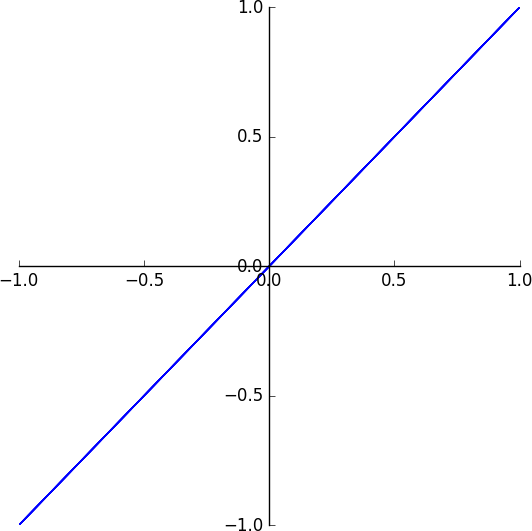
\includegraphics[scale=.2]{imagenes/modo_normal1.png}
 \end{center}
\end{wrapfigure}
 Los desplazamientos de las dos masas estan sobre la recta $y=x$, vale decir las masas se mueven perfectamente en fase.


 \begin{center}
   \animategraphics[controls, scale=.4]{15}{osciladores_acoplados/primero/modo1-}{0}{9}
 \end{center}





\noindent\textbf{Segundo modo normal}

\begin{lstlisting}
>>> x1=x.subs({A:0,B:0,C:1,D:0})
>>> y1=x1.diff(t,2)+2*x1
>>> plot_parametric(x1,y1,(t,0,10*pi))
\end{lstlisting}

\begin{wrapfigure}[6]{l}{5cm}
  \begin{center}
   \vspace{-.5cm}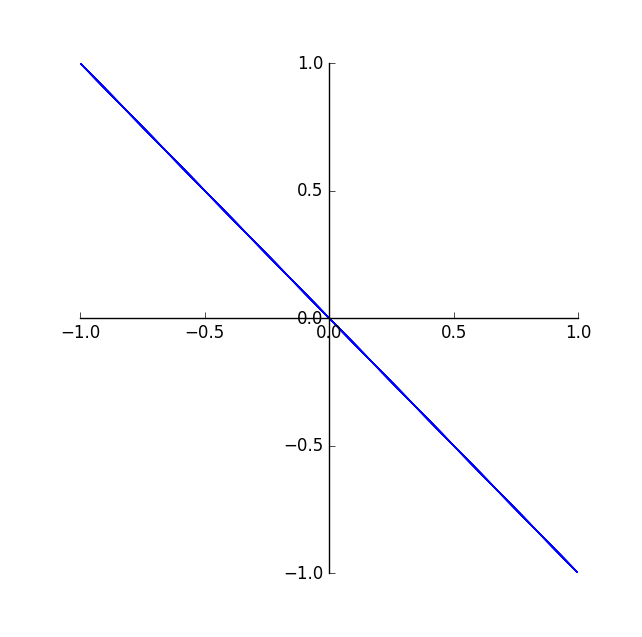
\includegraphics[scale=.2]{imagenes/modo_normal2.png}
 \end{center}
\end{wrapfigure}
Los desplazamientos de las dos masas estan sobre la recta $y=-x$, vale decir las masas se mueven perfectamente fuera de fase. Cuando una alcanza el desplazamiento negativo menor la otra alcanza el mayor positivo.


 \begin{center}
    \animategraphics[controls, scale=.4]{15}{osciladores_acoplados/segundo/modo2-}{0}{9}
 \end{center}



\noindent\textbf{Fuera de un modo normal}
\begin{lstlisting}
>>> x1=x.subs({A:1,B:0,C:1,D:0})
>>> y1=x1.diff(t,2)+2*x1
>>> plot_parametric(x1,y1,(t,0,10*pi))
\end{lstlisting}

\begin{wrapfigure}[6]{r}{5cm}
  \begin{center}
   \vspace{-.5cm}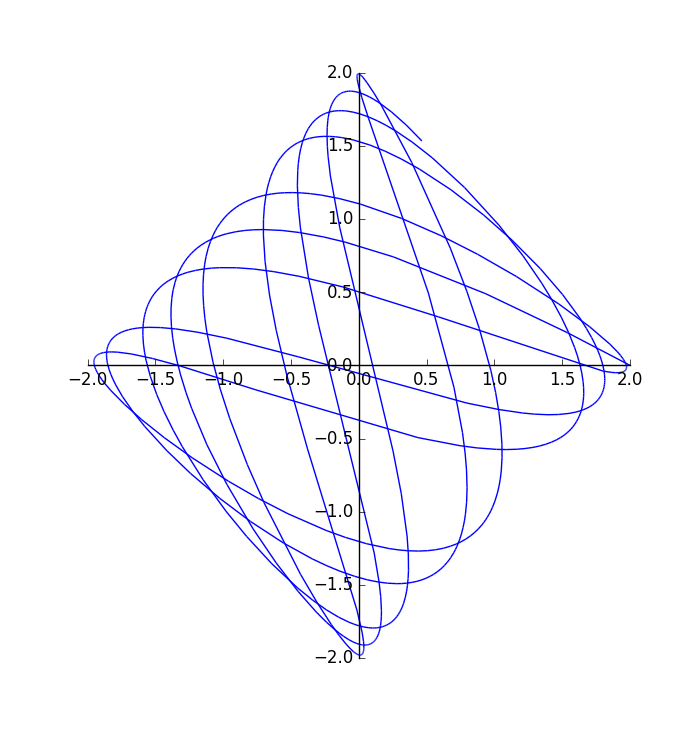
\includegraphics[scale=.2]{imagenes/lissajous.png}
   \caption{Curva de Lissajous}
 \end{center}
\end{wrapfigure}

Se obtienen gráficas  bonitas llamadas \href{http://es.wikipedia.org/wiki/Curva_de_Lissajous}{Curvas de Lissajous}, que fuera de los modos normales llenan densamente un cuadrado del plano.










\section{Métodos Operacionales}


El denominado \href{http://en.wikipedia.org/wiki/Operational_calculus}{Método Operacional} es una técnica iniciada por el ingeniero eléctrico  \href{http://es.wikipedia.org/wiki/Oliver_Heaviside}{Oliver Heavside} (1850-1925).

\begin{wrapfigure}[13]{r}{5cm}
  \begin{center}
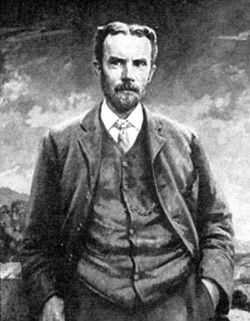
\includegraphics[scale=.8]{imagenes/Heaviside.jpg}
 \end{center}
 \caption{Oliver Heavside}
\end{wrapfigure}
Hemos mencionado que una ecuación lineal de orden $n$ con coeficientes constantes y  no homogénea se puede pensar como
\boxedeq{p(D)y=r(x),}{eq:lin_oper}
donde $p(D)=D^n+p_{n-1}D^{n-1}+\cdots+p_1D+ p_0$ es un operador diferencial polinomial.




La idea central del método es proceder desde una manera puramente formal, para afirmar que si $y$ resuelve
\eqref{eq:lin_oper} entonces
\boxedeq{y=\frac{1}{p(D)}r(x),}{eq:oper_inv}
Esto no parece más que un juego de símbolos del que no se puede desprender nada interesante. Vamos a ver que no es ese el caso.

El símbolo $1/p(D)$ debería ser interpretado como el operador inverso de $p(D)$. Por ejemplo, supongamos que $p(D)=D$. entonces $p(D)y=y'$. En este caso $1/p(D)$ puede ser definido como

\boxedeq{\frac{1}{p(D)}r=\int r(x)dx}{eq:oper_inv_int}

Si tuviesemos $p(D)=D-q$, $q\in\rr$, entonces $p(D)y=y'-qy$. En este caso, teniendo en mente que $y(x)=(1/p(D))r(x)$ debería resolver la ecuación lineal de primer orden $y'-qy=r(x)$, y por la fórmula explícita que obtuvimos para esta solución, es natural definir
\boxedeq{\frac{1}{p(D)}r=e^{qx}\int e^{-qx}r(x)dx}{eq:oper_inv_lin}

\subsection{Raíces simples}
Supongamos ahora que $p$ es un polinomio que se factoriza en monomios de primer orden
\[p(D)=(D-p_0)\cdots(D-p_k).\]
Siguiendo la línea de razonamiento aneterior
definimos
\boxedeq{\frac{1}{p(D)}r=\frac{1}{D-p_0}\left(\frac{1}{D-p_1}\left(\cdots\frac{1}{D-p_k}\left(r  \right)\cdots    \right)  \right)}{eq:oper_inv_fact}


\noindent\textbf{Problema.} Resolver  $y''-3y'+2y=xe^x$. Las cuentas las haremos con SymPy. Primero veamos si el polinomio se factoriza



\begin{lstlisting}
>>> var('D')
>>> p=D**2-3*D+2
>>> p.factor()
\end{lstlisting}

Vemos que $p(D)=(D-2)(D-1)$. Ahora programemos la fórmula \eqref{eq:oper_inv_lin} y usemosla para resolver la ecuación.
\begin{lstlisting}
>>> x=var('x')
>>> LinInv=lambda r,a: exp(a*x)* integrate(exp(-a*x)*r,x)
>>> LinInv(LinInv(x*exp(x),1),2)
\end{lstlisting}
Deducimos $y=\frac{e^{x}}{2} \left(- x^{2} - 2 x - 2\right)
$ es solución.



\subsubsection{Fracciones simples}
 Otra idea es descomponer $1/p(D)$ en fracciones simples. Suponiendo $p(D)=(D-p_0)\cdots(D-p_k)$, con $p_j$ raíces simples
\[\frac{1}{(D-p_0)\cdots(D-p_k)}=\left\{\frac{A_0}{(D-p_0)}+\cdots+\frac{A_k}{(D-p_k)}\right\}.\]
Como cada témino del miembro de la derecha lo tenemos definido, sólo tenemos que sumar cada uno de ellos. Reprocesemos con esta idea el  ejemplo de antes. La función \texttt{apart} de sympy hace descomposiciones en fracciones simples. En el caso del operador $p(D)=(D-2)(D-1)$ obtenemos descomposición en fracciones simples
\begin{lstlisting}
>> apart(1/p)
\end{lstlisting}

\[\frac{1}{p(D)}=-\frac{1}{D-1}+\frac{1}{D-2}.\]
 Entonces la siguiente expresión debería darnos una solución
\begin{lstlisting}
>>> LinInv(x*exp(x),2)-LinInv(x*exp(x),1)
\end{lstlisting}
Obviamente obtenemos la misma solución que obtuvimos antes.

\subsection{Series}
En algunas ocasiones es conveniente desarrollar en serie $1/p(D)$:
\boxedeq{\frac{1}{p(D)}r(x)=\left(a_0+a_1D+a_2D^2+\cdots \right)r(x).}{eq:des_serie}
Por ejemplo cuando $r$ es un polinomio, puesto que salvo una cantidad finita, todas las derivadas de orden $k$ de $r$ son cero.

\noindent\textbf{Ejemplo.} Resolver $y'''+2y''+y=x^4+2x+5$.
Como $r$ es un polinomio de grado 4, desarrollemos en serie $1/p(D)$ hasta ese orden

\begin{lstlisting}
>>> L=1/(1+2*D**2+D**3)
>>> L.series(D,0,5)
\end{lstlisting}
Obtenemos
\[\frac{1}{p(D)}=\frac{1}{1+2D^2+D^3}=
1 - 2 D^{2} - D^{3} + 4 D^{4} + \mathcal{O}\left(D^{5}\right).\]
Ahora el siguiente código  define el operador diferencial asociado a la expresión anterior
\begin{lstlisting}
>>> coeficientes=[Q.diff(D,j).subs(D,0)/factorial(j) for j in range(5)]
        def Q_op(f):
	return sum([coeficientes[j]*f.diff(x,j) for j in range(5)])
\end{lstlisting}

Evaluamos el segundo miembro de  \eqref{eq:des_serie} en $r(x)=x^4+2x+5$.
\begin{lstlisting}
>>> Q_op(x**4+2*x+5)
\end{lstlisting}
Llegamos a la solución
\[y=x^{4} - 24 x^{2} - 22 x + 101
\]

%\end{document}
